% !iTeXMac(input): POH.tex
\chapter{PERFORMANCE}
\label{perf-sec-number}
\vspace{\minitocspacebefore}
\minitoc
\cleardoublepage

%% following five commands to control the placement of figures on the pages
%% these values are changed for the Performance Section to allow room 
%% for two graphs on one page, with no text outside the figure.
\renewcommand{\textfraction}{0.0} 
\renewcommand{\topfraction}{1} 
\renewcommand{\bottomfraction}{1} 
\renewcommand{\floatpagefraction}{0.35} 
\setcounter{totalnumber}{5} 

\section{INTRODUCTION}
Most of the information in the Performance Section is preliminary, based on analysis of
 data from Van's Aircraft or the CAFE Foundation.
The section will be completely revised once performance flight testing has been completed.
\clearpage


% Temperature Conversion Chart
\begin{figure}[t]
% \addcontentsline{toc}{section}{Figure \ref{Temp-comp-chart} Temperature Conversion Chart}
\addcontentsline{toc}{section}{TEMPERATURE CONVERSION CHART}
\centering{
  \begin{perfhdr}TEMPERATURE CONVERSION CHART\\
  \end{perfhdr}
  \begin{center}
  % GNUPLOT: LaTeX picture with Postscript
\begingroup
  \makeatletter
  \providecommand\color[2][]{%
    \GenericError{(gnuplot) \space\space\space\@spaces}{%
      Package color not loaded in conjunction with
      terminal option `colourtext'%
    }{See the gnuplot documentation for explanation.%
    }{Either use 'blacktext' in gnuplot or load the package
      color.sty in LaTeX.}%
    \renewcommand\color[2][]{}%
  }%
  \providecommand\includegraphics[2][]{%
    \GenericError{(gnuplot) \space\space\space\@spaces}{%
      Package graphicx or graphics not loaded%
    }{See the gnuplot documentation for explanation.%
    }{The gnuplot epslatex terminal needs graphicx.sty or graphics.sty.}%
    \renewcommand\includegraphics[2][]{}%
  }%
  \providecommand\rotatebox[2]{#2}%
  \@ifundefined{ifGPcolor}{%
    \newif\ifGPcolor
    \GPcolorfalse
  }{}%
  \@ifundefined{ifGPblacktext}{%
    \newif\ifGPblacktext
    \GPblacktexttrue
  }{}%
  % define a \g@addto@macro without @ in the name:
  \let\gplgaddtomacro\g@addto@macro
  % define empty templates for all commands taking text:
  \gdef\gplbacktext{}%
  \gdef\gplfronttext{}%
  \makeatother
  \ifGPblacktext
    % no textcolor at all
    \def\colorrgb#1{}%
    \def\colorgray#1{}%
  \else
    % gray or color?
    \ifGPcolor
      \def\colorrgb#1{\color[rgb]{#1}}%
      \def\colorgray#1{\color[gray]{#1}}%
      \expandafter\def\csname LTw\endcsname{\color{white}}%
      \expandafter\def\csname LTb\endcsname{\color{black}}%
      \expandafter\def\csname LTa\endcsname{\color{black}}%
      \expandafter\def\csname LT0\endcsname{\color[rgb]{1,0,0}}%
      \expandafter\def\csname LT1\endcsname{\color[rgb]{0,1,0}}%
      \expandafter\def\csname LT2\endcsname{\color[rgb]{0,0,1}}%
      \expandafter\def\csname LT3\endcsname{\color[rgb]{1,0,1}}%
      \expandafter\def\csname LT4\endcsname{\color[rgb]{0,1,1}}%
      \expandafter\def\csname LT5\endcsname{\color[rgb]{1,1,0}}%
      \expandafter\def\csname LT6\endcsname{\color[rgb]{0,0,0}}%
      \expandafter\def\csname LT7\endcsname{\color[rgb]{1,0.3,0}}%
      \expandafter\def\csname LT8\endcsname{\color[rgb]{0.5,0.5,0.5}}%
    \else
      % gray
      \def\colorrgb#1{\color{black}}%
      \def\colorgray#1{\color[gray]{#1}}%
      \expandafter\def\csname LTw\endcsname{\color{white}}%
      \expandafter\def\csname LTb\endcsname{\color{black}}%
      \expandafter\def\csname LTa\endcsname{\color{black}}%
      \expandafter\def\csname LT0\endcsname{\color{black}}%
      \expandafter\def\csname LT1\endcsname{\color{black}}%
      \expandafter\def\csname LT2\endcsname{\color{black}}%
      \expandafter\def\csname LT3\endcsname{\color{black}}%
      \expandafter\def\csname LT4\endcsname{\color{black}}%
      \expandafter\def\csname LT5\endcsname{\color{black}}%
      \expandafter\def\csname LT6\endcsname{\color{black}}%
      \expandafter\def\csname LT7\endcsname{\color{black}}%
      \expandafter\def\csname LT8\endcsname{\color{black}}%
    \fi
  \fi
  \setlength{\unitlength}{0.0500bp}%
  \begin{picture}(7200.00,10080.00)%
    \gplgaddtomacro\gplbacktext{%
      \csname LTb\endcsname%
      \put(1078,704){\makebox(0,0)[r]{\strut{}-40}}%
      \csname LTb\endcsname%
      \put(1078,1843){\makebox(0,0)[r]{\strut{}-20}}%
      \csname LTb\endcsname%
      \put(1078,2982){\makebox(0,0)[r]{\strut{} 0}}%
      \csname LTb\endcsname%
      \put(1078,4120){\makebox(0,0)[r]{\strut{} 20}}%
      \csname LTb\endcsname%
      \put(1078,5259){\makebox(0,0)[r]{\strut{} 40}}%
      \csname LTb\endcsname%
      \put(1078,6398){\makebox(0,0)[r]{\strut{} 60}}%
      \csname LTb\endcsname%
      \put(1078,7537){\makebox(0,0)[r]{\strut{} 80}}%
      \csname LTb\endcsname%
      \put(1078,8675){\makebox(0,0)[r]{\strut{} 100}}%
      \csname LTb\endcsname%
      \put(1078,9814){\makebox(0,0)[r]{\strut{} 120}}%
      \csname LTb\endcsname%
      \put(1210,484){\makebox(0,0){\strut{}-40}}%
      \csname LTb\endcsname%
      \put(2342,484){\makebox(0,0){\strut{}-20}}%
      \csname LTb\endcsname%
      \put(3474,484){\makebox(0,0){\strut{} 0}}%
      \csname LTb\endcsname%
      \put(4605,484){\makebox(0,0){\strut{} 20}}%
      \csname LTb\endcsname%
      \put(5737,484){\makebox(0,0){\strut{} 40}}%
      \csname LTb\endcsname%
      \put(6869,484){\makebox(0,0){\strut{} 60}}%
      \put(308,5259){\rotatebox{-270}{\makebox(0,0){\strut{}Temperature (\textdegree F)}}}%
      \put(4039,154){\makebox(0,0){\strut{}Temperature (\textdegree C)}}%
    }%
    \gplgaddtomacro\gplfronttext{%
    }%
    \gplbacktext
    \put(0,0){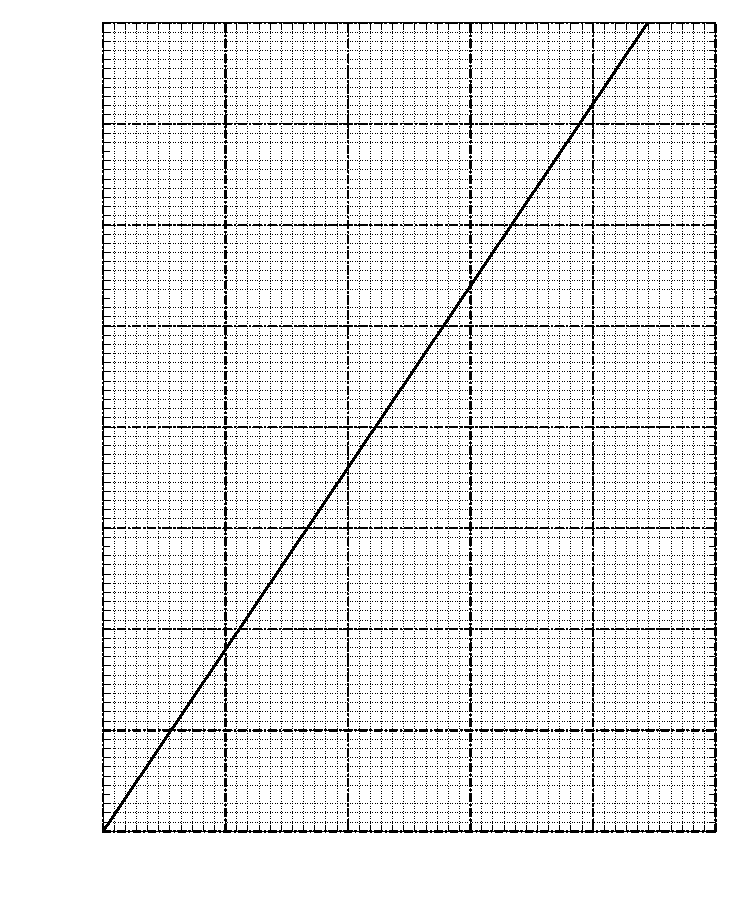
\includegraphics{../graphs/temp_conv}}%
    \gplfronttext
  \end{picture}%
\endgroup
\end{center}  % for gnuplot epslatex, latex or pslatex mode
}
\caption{Temperature Conversion Chart}
\label{Temp-comp-chart}
\end{figure}

        % Temperature Conversion Chart
% Weight Conversion Chart
\begin{figure}[t]
% \addcontentsline{toc}{section}{Figure \ref{Weight-comp-chart} Weight Conversion Chart}
\addcontentsline{toc}{section}{WEIGHT CONVERSION CHART}
\centering{
  \begin{perfhdr}WEIGHT CONVERSION CHART\\
  \end{perfhdr}
  \begin{center}
  % GNUPLOT: LaTeX picture with Postscript
\begingroup
  \makeatletter
  \providecommand\color[2][]{%
    \GenericError{(gnuplot) \space\space\space\@spaces}{%
      Package color not loaded in conjunction with
      terminal option `colourtext'%
    }{See the gnuplot documentation for explanation.%
    }{Either use 'blacktext' in gnuplot or load the package
      color.sty in LaTeX.}%
    \renewcommand\color[2][]{}%
  }%
  \providecommand\includegraphics[2][]{%
    \GenericError{(gnuplot) \space\space\space\@spaces}{%
      Package graphicx or graphics not loaded%
    }{See the gnuplot documentation for explanation.%
    }{The gnuplot epslatex terminal needs graphicx.sty or graphics.sty.}%
    \renewcommand\includegraphics[2][]{}%
  }%
  \providecommand\rotatebox[2]{#2}%
  \@ifundefined{ifGPcolor}{%
    \newif\ifGPcolor
    \GPcolorfalse
  }{}%
  \@ifundefined{ifGPblacktext}{%
    \newif\ifGPblacktext
    \GPblacktexttrue
  }{}%
  % define a \g@addto@macro without @ in the name:
  \let\gplgaddtomacro\g@addto@macro
  % define empty templates for all commands taking text:
  \gdef\gplbacktext{}%
  \gdef\gplfronttext{}%
  \makeatother
  \ifGPblacktext
    % no textcolor at all
    \def\colorrgb#1{}%
    \def\colorgray#1{}%
  \else
    % gray or color?
    \ifGPcolor
      \def\colorrgb#1{\color[rgb]{#1}}%
      \def\colorgray#1{\color[gray]{#1}}%
      \expandafter\def\csname LTw\endcsname{\color{white}}%
      \expandafter\def\csname LTb\endcsname{\color{black}}%
      \expandafter\def\csname LTa\endcsname{\color{black}}%
      \expandafter\def\csname LT0\endcsname{\color[rgb]{1,0,0}}%
      \expandafter\def\csname LT1\endcsname{\color[rgb]{0,1,0}}%
      \expandafter\def\csname LT2\endcsname{\color[rgb]{0,0,1}}%
      \expandafter\def\csname LT3\endcsname{\color[rgb]{1,0,1}}%
      \expandafter\def\csname LT4\endcsname{\color[rgb]{0,1,1}}%
      \expandafter\def\csname LT5\endcsname{\color[rgb]{1,1,0}}%
      \expandafter\def\csname LT6\endcsname{\color[rgb]{0,0,0}}%
      \expandafter\def\csname LT7\endcsname{\color[rgb]{1,0.3,0}}%
      \expandafter\def\csname LT8\endcsname{\color[rgb]{0.5,0.5,0.5}}%
    \else
      % gray
      \def\colorrgb#1{\color{black}}%
      \def\colorgray#1{\color[gray]{#1}}%
      \expandafter\def\csname LTw\endcsname{\color{white}}%
      \expandafter\def\csname LTb\endcsname{\color{black}}%
      \expandafter\def\csname LTa\endcsname{\color{black}}%
      \expandafter\def\csname LT0\endcsname{\color{black}}%
      \expandafter\def\csname LT1\endcsname{\color{black}}%
      \expandafter\def\csname LT2\endcsname{\color{black}}%
      \expandafter\def\csname LT3\endcsname{\color{black}}%
      \expandafter\def\csname LT4\endcsname{\color{black}}%
      \expandafter\def\csname LT5\endcsname{\color{black}}%
      \expandafter\def\csname LT6\endcsname{\color{black}}%
      \expandafter\def\csname LT7\endcsname{\color{black}}%
      \expandafter\def\csname LT8\endcsname{\color{black}}%
    \fi
  \fi
  \setlength{\unitlength}{0.0500bp}%
  \begin{picture}(7200.00,10080.00)%
    \gplgaddtomacro\gplbacktext{%
      \csname LTb\endcsname%
      \put(1210,704){\makebox(0,0)[r]{\strut{} 0}}%
      \csname LTb\endcsname%
      \put(1210,1615){\makebox(0,0)[r]{\strut{} 200}}%
      \csname LTb\endcsname%
      \put(1210,2526){\makebox(0,0)[r]{\strut{} 400}}%
      \csname LTb\endcsname%
      \put(1210,3437){\makebox(0,0)[r]{\strut{} 600}}%
      \csname LTb\endcsname%
      \put(1210,4348){\makebox(0,0)[r]{\strut{} 800}}%
      \csname LTb\endcsname%
      \put(1210,5259){\makebox(0,0)[r]{\strut{} 1000}}%
      \csname LTb\endcsname%
      \put(1210,6170){\makebox(0,0)[r]{\strut{} 1200}}%
      \csname LTb\endcsname%
      \put(1210,7081){\makebox(0,0)[r]{\strut{} 1400}}%
      \csname LTb\endcsname%
      \put(1210,7992){\makebox(0,0)[r]{\strut{} 1600}}%
      \csname LTb\endcsname%
      \put(1210,8903){\makebox(0,0)[r]{\strut{} 1800}}%
      \csname LTb\endcsname%
      \put(1210,9814){\makebox(0,0)[r]{\strut{} 2000}}%
      \csname LTb\endcsname%
      \put(1342,484){\makebox(0,0){\strut{} 0}}%
      \csname LTb\endcsname%
      \put(1956,484){\makebox(0,0){\strut{} 100}}%
      \csname LTb\endcsname%
      \put(2570,484){\makebox(0,0){\strut{} 200}}%
      \csname LTb\endcsname%
      \put(3184,484){\makebox(0,0){\strut{} 300}}%
      \csname LTb\endcsname%
      \put(3798,484){\makebox(0,0){\strut{} 400}}%
      \csname LTb\endcsname%
      \put(4413,484){\makebox(0,0){\strut{} 500}}%
      \csname LTb\endcsname%
      \put(5027,484){\makebox(0,0){\strut{} 600}}%
      \csname LTb\endcsname%
      \put(5641,484){\makebox(0,0){\strut{} 700}}%
      \csname LTb\endcsname%
      \put(6255,484){\makebox(0,0){\strut{} 800}}%
      \csname LTb\endcsname%
      \put(6869,484){\makebox(0,0){\strut{} 900}}%
      \put(308,5259){\rotatebox{-270}{\makebox(0,0){\strut{}Weight (lb)}}}%
      \put(4105,154){\makebox(0,0){\strut{}Mass (kg)}}%
    }%
    \gplgaddtomacro\gplfronttext{%
    }%
    \gplbacktext
    \put(0,0){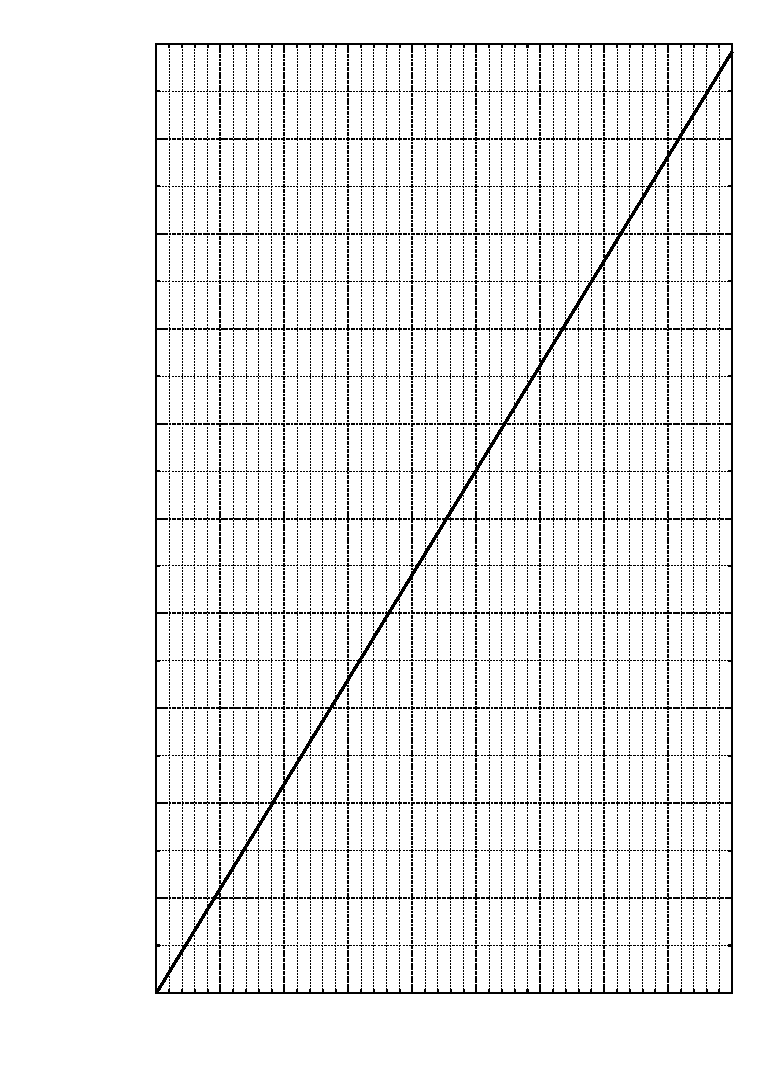
\includegraphics{../graphs/wt_conv}}%
    \gplfronttext
  \end{picture}%
\endgroup
\end{center}  % for gnuplot epslatex, latex or pslatex mode
}
\caption{Weight Conversion Chart}
\label{Weight-comp-chart}
\end{figure}

      % Weight Conversion Chart
% Volume Conversion Chart
\begin{figure}[t]
% \addcontentsline{toc}{section}{Figure \ref{Weight-comp-chart} Volume Conversion Chart}
\addcontentsline{toc}{section}{VOLUME CONVERSION CHART}
\centering{
  \begin{perfhdr}VOLUME CONVERSION CHART\\
  \end{perfhdr}
  \begin{center}
  % GNUPLOT: LaTeX picture with Postscript
\begingroup
  \makeatletter
  \providecommand\color[2][]{%
    \GenericError{(gnuplot) \space\space\space\@spaces}{%
      Package color not loaded in conjunction with
      terminal option `colourtext'%
    }{See the gnuplot documentation for explanation.%
    }{Either use 'blacktext' in gnuplot or load the package
      color.sty in LaTeX.}%
    \renewcommand\color[2][]{}%
  }%
  \providecommand\includegraphics[2][]{%
    \GenericError{(gnuplot) \space\space\space\@spaces}{%
      Package graphicx or graphics not loaded%
    }{See the gnuplot documentation for explanation.%
    }{The gnuplot epslatex terminal needs graphicx.sty or graphics.sty.}%
    \renewcommand\includegraphics[2][]{}%
  }%
  \providecommand\rotatebox[2]{#2}%
  \@ifundefined{ifGPcolor}{%
    \newif\ifGPcolor
    \GPcolorfalse
  }{}%
  \@ifundefined{ifGPblacktext}{%
    \newif\ifGPblacktext
    \GPblacktexttrue
  }{}%
  % define a \g@addto@macro without @ in the name:
  \let\gplgaddtomacro\g@addto@macro
  % define empty templates for all commands taking text:
  \gdef\gplbacktext{}%
  \gdef\gplfronttext{}%
  \makeatother
  \ifGPblacktext
    % no textcolor at all
    \def\colorrgb#1{}%
    \def\colorgray#1{}%
  \else
    % gray or color?
    \ifGPcolor
      \def\colorrgb#1{\color[rgb]{#1}}%
      \def\colorgray#1{\color[gray]{#1}}%
      \expandafter\def\csname LTw\endcsname{\color{white}}%
      \expandafter\def\csname LTb\endcsname{\color{black}}%
      \expandafter\def\csname LTa\endcsname{\color{black}}%
      \expandafter\def\csname LT0\endcsname{\color[rgb]{1,0,0}}%
      \expandafter\def\csname LT1\endcsname{\color[rgb]{0,1,0}}%
      \expandafter\def\csname LT2\endcsname{\color[rgb]{0,0,1}}%
      \expandafter\def\csname LT3\endcsname{\color[rgb]{1,0,1}}%
      \expandafter\def\csname LT4\endcsname{\color[rgb]{0,1,1}}%
      \expandafter\def\csname LT5\endcsname{\color[rgb]{1,1,0}}%
      \expandafter\def\csname LT6\endcsname{\color[rgb]{0,0,0}}%
      \expandafter\def\csname LT7\endcsname{\color[rgb]{1,0.3,0}}%
      \expandafter\def\csname LT8\endcsname{\color[rgb]{0.5,0.5,0.5}}%
    \else
      % gray
      \def\colorrgb#1{\color{black}}%
      \def\colorgray#1{\color[gray]{#1}}%
      \expandafter\def\csname LTw\endcsname{\color{white}}%
      \expandafter\def\csname LTb\endcsname{\color{black}}%
      \expandafter\def\csname LTa\endcsname{\color{black}}%
      \expandafter\def\csname LT0\endcsname{\color{black}}%
      \expandafter\def\csname LT1\endcsname{\color{black}}%
      \expandafter\def\csname LT2\endcsname{\color{black}}%
      \expandafter\def\csname LT3\endcsname{\color{black}}%
      \expandafter\def\csname LT4\endcsname{\color{black}}%
      \expandafter\def\csname LT5\endcsname{\color{black}}%
      \expandafter\def\csname LT6\endcsname{\color{black}}%
      \expandafter\def\csname LT7\endcsname{\color{black}}%
      \expandafter\def\csname LT8\endcsname{\color{black}}%
    \fi
  \fi
  \setlength{\unitlength}{0.0500bp}%
  \begin{picture}(7200.00,10080.00)%
    \gplgaddtomacro\gplbacktext{%
      \csname LTb\endcsname%
      \put(1078,704){\makebox(0,0)[r]{\strut{} 0}}%
      \csname LTb\endcsname%
      \put(1078,1615){\makebox(0,0)[r]{\strut{} 20}}%
      \csname LTb\endcsname%
      \put(1078,2526){\makebox(0,0)[r]{\strut{} 40}}%
      \csname LTb\endcsname%
      \put(1078,3437){\makebox(0,0)[r]{\strut{} 60}}%
      \csname LTb\endcsname%
      \put(1078,4348){\makebox(0,0)[r]{\strut{} 80}}%
      \csname LTb\endcsname%
      \put(1078,5259){\makebox(0,0)[r]{\strut{} 100}}%
      \csname LTb\endcsname%
      \put(1078,6170){\makebox(0,0)[r]{\strut{} 120}}%
      \csname LTb\endcsname%
      \put(1078,7081){\makebox(0,0)[r]{\strut{} 140}}%
      \csname LTb\endcsname%
      \put(1078,7992){\makebox(0,0)[r]{\strut{} 160}}%
      \csname LTb\endcsname%
      \put(1078,8903){\makebox(0,0)[r]{\strut{} 180}}%
      \csname LTb\endcsname%
      \put(1078,9814){\makebox(0,0)[r]{\strut{} 200}}%
      \csname LTb\endcsname%
      \put(1210,484){\makebox(0,0){\strut{} 0}}%
      \csname LTb\endcsname%
      \put(2342,484){\makebox(0,0){\strut{} 10}}%
      \csname LTb\endcsname%
      \put(3474,484){\makebox(0,0){\strut{} 20}}%
      \csname LTb\endcsname%
      \put(4605,484){\makebox(0,0){\strut{} 30}}%
      \csname LTb\endcsname%
      \put(5737,484){\makebox(0,0){\strut{} 40}}%
      \csname LTb\endcsname%
      \put(6869,484){\makebox(0,0){\strut{} 50}}%
      \put(308,5259){\rotatebox{-270}{\makebox(0,0){\strut{}Volume (l)}}}%
      \put(4039,154){\makebox(0,0){\strut{}Volume (USG)}}%
    }%
    \gplgaddtomacro\gplfronttext{%
    }%
    \gplbacktext
    \put(0,0){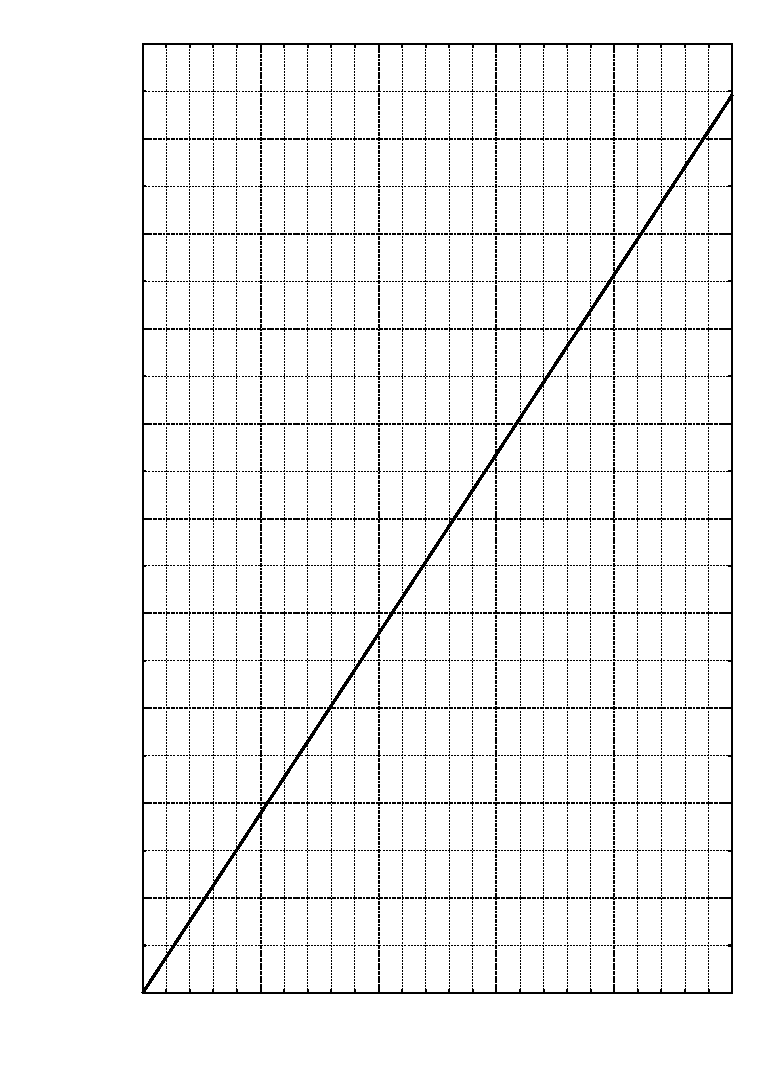
\includegraphics{../graphs/vol_conv}}%
    \gplfronttext
  \end{picture}%
\endgroup
\end{center}  % for gnuplot epslatex, latex or pslatex mode
}
\caption{Volume Conversion Chart}
\label{Volume-comp-chart}
\end{figure}

         % Volume Conversion Chart
% Static Source Position Error, Airspeed Chart
%% try boxedminipage.sty to get box around figure, to help separate two figures if there are more than one per page
\begin{figure}[t]
% \addcontentsline{toc}{section}{Figure \ref{SSEC-spd-error} Position Error --- Airspeed --- Flaps Retracted}
\addcontentsline{toc}{section}{POSITION ERROR --- AIRSPEED --- FLAPS RETRACTED}
\centering{
  \begin{perfhdr}POSITION ERROR --- AIRSPEED\\
  FLAPS RETRACTED\\
  \end{perfhdr}

  \centering{\begin{minipage}{5in}\begin{tabbing}
  EFIS Make - Model:aaaaa\= \kill
  Weight:\>1400 lb\\
  Flaps:\>Retracted\\
  Date of flight tests:\>14 \& 19 Nov 2008
  \end{tabbing}\end{minipage}}
  \begin{center}
  % GNUPLOT: LaTeX picture with Postscript
\begingroup
  \makeatletter
  \providecommand\color[2][]{%
    \GenericError{(gnuplot) \space\space\space\@spaces}{%
      Package color not loaded in conjunction with
      terminal option `colourtext'%
    }{See the gnuplot documentation for explanation.%
    }{Either use 'blacktext' in gnuplot or load the package
      color.sty in LaTeX.}%
    \renewcommand\color[2][]{}%
  }%
  \providecommand\includegraphics[2][]{%
    \GenericError{(gnuplot) \space\space\space\@spaces}{%
      Package graphicx or graphics not loaded%
    }{See the gnuplot documentation for explanation.%
    }{The gnuplot epslatex terminal needs graphicx.sty or graphics.sty.}%
    \renewcommand\includegraphics[2][]{}%
  }%
  \providecommand\rotatebox[2]{#2}%
  \@ifundefined{ifGPcolor}{%
    \newif\ifGPcolor
    \GPcolorfalse
  }{}%
  \@ifundefined{ifGPblacktext}{%
    \newif\ifGPblacktext
    \GPblacktexttrue
  }{}%
  % define a \g@addto@macro without @ in the name:
  \let\gplgaddtomacro\g@addto@macro
  % define empty templates for all commands taking text:
  \gdef\gplbacktext{}%
  \gdef\gplfronttext{}%
  \makeatother
  \ifGPblacktext
    % no textcolor at all
    \def\colorrgb#1{}%
    \def\colorgray#1{}%
  \else
    % gray or color?
    \ifGPcolor
      \def\colorrgb#1{\color[rgb]{#1}}%
      \def\colorgray#1{\color[gray]{#1}}%
      \expandafter\def\csname LTw\endcsname{\color{white}}%
      \expandafter\def\csname LTb\endcsname{\color{black}}%
      \expandafter\def\csname LTa\endcsname{\color{black}}%
      \expandafter\def\csname LT0\endcsname{\color[rgb]{1,0,0}}%
      \expandafter\def\csname LT1\endcsname{\color[rgb]{0,1,0}}%
      \expandafter\def\csname LT2\endcsname{\color[rgb]{0,0,1}}%
      \expandafter\def\csname LT3\endcsname{\color[rgb]{1,0,1}}%
      \expandafter\def\csname LT4\endcsname{\color[rgb]{0,1,1}}%
      \expandafter\def\csname LT5\endcsname{\color[rgb]{1,1,0}}%
      \expandafter\def\csname LT6\endcsname{\color[rgb]{0,0,0}}%
      \expandafter\def\csname LT7\endcsname{\color[rgb]{1,0.3,0}}%
      \expandafter\def\csname LT8\endcsname{\color[rgb]{0.5,0.5,0.5}}%
    \else
      % gray
      \def\colorrgb#1{\color{black}}%
      \def\colorgray#1{\color[gray]{#1}}%
      \expandafter\def\csname LTw\endcsname{\color{white}}%
      \expandafter\def\csname LTb\endcsname{\color{black}}%
      \expandafter\def\csname LTa\endcsname{\color{black}}%
      \expandafter\def\csname LT0\endcsname{\color{black}}%
      \expandafter\def\csname LT1\endcsname{\color{black}}%
      \expandafter\def\csname LT2\endcsname{\color{black}}%
      \expandafter\def\csname LT3\endcsname{\color{black}}%
      \expandafter\def\csname LT4\endcsname{\color{black}}%
      \expandafter\def\csname LT5\endcsname{\color{black}}%
      \expandafter\def\csname LT6\endcsname{\color{black}}%
      \expandafter\def\csname LT7\endcsname{\color{black}}%
      \expandafter\def\csname LT8\endcsname{\color{black}}%
    \fi
  \fi
  \setlength{\unitlength}{0.0500bp}%
  \begin{picture}(7200.00,5040.00)%
    \gplgaddtomacro\gplbacktext{%
      \csname LTb\endcsname%
      \put(1078,704){\makebox(0,0)[r]{\strut{}-5}}%
      \csname LTb\endcsname%
      \put(1078,1038){\makebox(0,0)[r]{\strut{}-4.5}}%
      \csname LTb\endcsname%
      \put(1078,1372){\makebox(0,0)[r]{\strut{}-4}}%
      \csname LTb\endcsname%
      \put(1078,1706){\makebox(0,0)[r]{\strut{}-3.5}}%
      \csname LTb\endcsname%
      \put(1078,2040){\makebox(0,0)[r]{\strut{}-3}}%
      \csname LTb\endcsname%
      \put(1078,2374){\makebox(0,0)[r]{\strut{}-2.5}}%
      \csname LTb\endcsname%
      \put(1078,2709){\makebox(0,0)[r]{\strut{}-2}}%
      \csname LTb\endcsname%
      \put(1078,3043){\makebox(0,0)[r]{\strut{}-1.5}}%
      \csname LTb\endcsname%
      \put(1078,3377){\makebox(0,0)[r]{\strut{}-1}}%
      \csname LTb\endcsname%
      \put(1078,3711){\makebox(0,0)[r]{\strut{}-0.5}}%
      \csname LTb\endcsname%
      \put(1078,4045){\makebox(0,0)[r]{\strut{} 0}}%
      \csname LTb\endcsname%
      \put(1078,4379){\makebox(0,0)[r]{\strut{} 0.5}}%
      \csname LTb\endcsname%
      \put(1210,484){\makebox(0,0){\strut{} 50}}%
      \csname LTb\endcsname%
      \put(2625,484){\makebox(0,0){\strut{} 100}}%
      \csname LTb\endcsname%
      \put(4040,484){\makebox(0,0){\strut{} 150}}%
      \csname LTb\endcsname%
      \put(5454,484){\makebox(0,0){\strut{} 200}}%
      \csname LTb\endcsname%
      \put(6869,484){\makebox(0,0){\strut{} 250}}%
      \put(308,2541){\rotatebox{-270}{\makebox(0,0){\strut{}Position Error in Airspeed (kt)}}}%
      \put(4039,154){\makebox(0,0){\strut{}IAS - instrument corrected (kt)}}%
      \put(4039,4709){\makebox(0,0){\strut{}Static Source Position Error - Airspeed - Flaps Retracted}}%
    }%
    \gplgaddtomacro\gplfronttext{%
      \put(3332,2207){\makebox(0,0){\strut{}CAS = IAS + Error}}%
      \put(3332,1873){\makebox(0,0){\strut{}ASI Instrument Error Assumed to be Zero}}%
    }%
    \gplbacktext
    \put(0,0){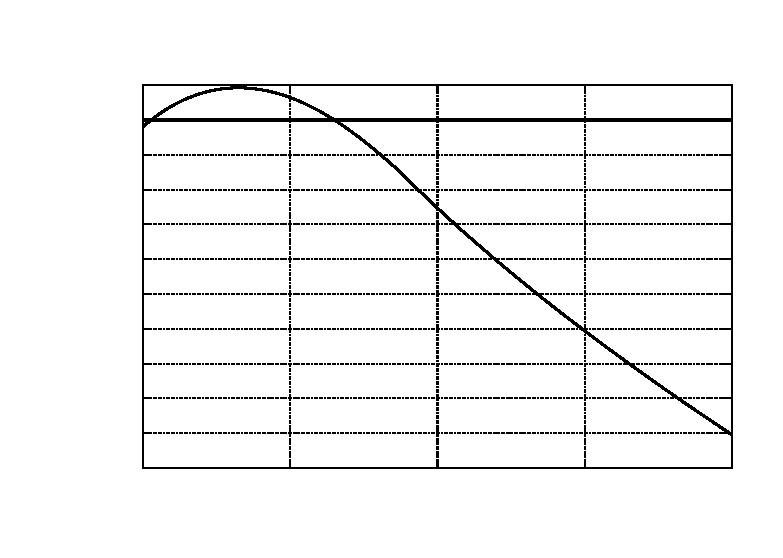
\includegraphics{../graphs/ias_error_no_inst_corr_flaps_up}}%
    \gplfronttext
  \end{picture}%
\endgroup
\end{center}  % for gnuplot epslatex, latex or pslatex mode
}
\caption{Position Error --- Airspeed --- Flaps Retracted}
\label{SSEC-spd-error}
\end{figure}

               % Static Source Position Error, Airspeed Chart
% Static Source Position Error, Altitude Chart
%% try boxedminipage.sty to get box around figure, to help separate two figures if there are more than one per page
\begin{figure}[t]
% \addcontentsline{toc}{section}{Figure \ref{SSEC-alt-error} Position Error --- Altitude --- Flaps Retracted}
\addcontentsline{toc}{section}{POSITION ERROR --- ALTITUDE --- FLAPS RETRACTED}
\centering{
  \begin{perfhdr}POSITION ERROR --- ALTITUDE\\
  FLAPS RETRACTED\\
  \end{perfhdr}

  \centering{\begin{minipage}{5in}\begin{tabbing}
  EFIS Make - Model:aaaaa\= \kill
  Weight:\>1600 lb\\
  Flaps:\>Retracted\\
  Date of flight tests:\>14 \& 19 Nov 2008
  \end{tabbing}\end{minipage}}
  \begin{center}
  % GNUPLOT: LaTeX picture with Postscript
\begingroup
  \makeatletter
  \providecommand\color[2][]{%
    \GenericError{(gnuplot) \space\space\space\@spaces}{%
      Package color not loaded in conjunction with
      terminal option `colourtext'%
    }{See the gnuplot documentation for explanation.%
    }{Either use 'blacktext' in gnuplot or load the package
      color.sty in LaTeX.}%
    \renewcommand\color[2][]{}%
  }%
  \providecommand\includegraphics[2][]{%
    \GenericError{(gnuplot) \space\space\space\@spaces}{%
      Package graphicx or graphics not loaded%
    }{See the gnuplot documentation for explanation.%
    }{The gnuplot epslatex terminal needs graphicx.sty or graphics.sty.}%
    \renewcommand\includegraphics[2][]{}%
  }%
  \providecommand\rotatebox[2]{#2}%
  \@ifundefined{ifGPcolor}{%
    \newif\ifGPcolor
    \GPcolorfalse
  }{}%
  \@ifundefined{ifGPblacktext}{%
    \newif\ifGPblacktext
    \GPblacktexttrue
  }{}%
  % define a \g@addto@macro without @ in the name:
  \let\gplgaddtomacro\g@addto@macro
  % define empty templates for all commands taking text:
  \gdef\gplbacktext{}%
  \gdef\gplfronttext{}%
  \makeatother
  \ifGPblacktext
    % no textcolor at all
    \def\colorrgb#1{}%
    \def\colorgray#1{}%
  \else
    % gray or color?
    \ifGPcolor
      \def\colorrgb#1{\color[rgb]{#1}}%
      \def\colorgray#1{\color[gray]{#1}}%
      \expandafter\def\csname LTw\endcsname{\color{white}}%
      \expandafter\def\csname LTb\endcsname{\color{black}}%
      \expandafter\def\csname LTa\endcsname{\color{black}}%
      \expandafter\def\csname LT0\endcsname{\color[rgb]{1,0,0}}%
      \expandafter\def\csname LT1\endcsname{\color[rgb]{0,1,0}}%
      \expandafter\def\csname LT2\endcsname{\color[rgb]{0,0,1}}%
      \expandafter\def\csname LT3\endcsname{\color[rgb]{1,0,1}}%
      \expandafter\def\csname LT4\endcsname{\color[rgb]{0,1,1}}%
      \expandafter\def\csname LT5\endcsname{\color[rgb]{1,1,0}}%
      \expandafter\def\csname LT6\endcsname{\color[rgb]{0,0,0}}%
      \expandafter\def\csname LT7\endcsname{\color[rgb]{1,0.3,0}}%
      \expandafter\def\csname LT8\endcsname{\color[rgb]{0.5,0.5,0.5}}%
    \else
      % gray
      \def\colorrgb#1{\color{black}}%
      \def\colorgray#1{\color[gray]{#1}}%
      \expandafter\def\csname LTw\endcsname{\color{white}}%
      \expandafter\def\csname LTb\endcsname{\color{black}}%
      \expandafter\def\csname LTa\endcsname{\color{black}}%
      \expandafter\def\csname LT0\endcsname{\color{black}}%
      \expandafter\def\csname LT1\endcsname{\color{black}}%
      \expandafter\def\csname LT2\endcsname{\color{black}}%
      \expandafter\def\csname LT3\endcsname{\color{black}}%
      \expandafter\def\csname LT4\endcsname{\color{black}}%
      \expandafter\def\csname LT5\endcsname{\color{black}}%
      \expandafter\def\csname LT6\endcsname{\color{black}}%
      \expandafter\def\csname LT7\endcsname{\color{black}}%
      \expandafter\def\csname LT8\endcsname{\color{black}}%
    \fi
  \fi
  \setlength{\unitlength}{0.0500bp}%
  \begin{picture}(7200.00,5040.00)%
    \gplgaddtomacro\gplbacktext{%
      \csname LTb\endcsname%
      \put(946,704){\makebox(0,0)[r]{\strut{}-90}}%
      \csname LTb\endcsname%
      \put(946,1072){\makebox(0,0)[r]{\strut{}-80}}%
      \csname LTb\endcsname%
      \put(946,1439){\makebox(0,0)[r]{\strut{}-70}}%
      \csname LTb\endcsname%
      \put(946,1807){\makebox(0,0)[r]{\strut{}-60}}%
      \csname LTb\endcsname%
      \put(946,2174){\makebox(0,0)[r]{\strut{}-50}}%
      \csname LTb\endcsname%
      \put(946,2542){\makebox(0,0)[r]{\strut{}-40}}%
      \csname LTb\endcsname%
      \put(946,2909){\makebox(0,0)[r]{\strut{}-30}}%
      \csname LTb\endcsname%
      \put(946,3277){\makebox(0,0)[r]{\strut{}-20}}%
      \csname LTb\endcsname%
      \put(946,3644){\makebox(0,0)[r]{\strut{}-10}}%
      \csname LTb\endcsname%
      \put(946,4012){\makebox(0,0)[r]{\strut{} 0}}%
      \csname LTb\endcsname%
      \put(946,4379){\makebox(0,0)[r]{\strut{} 10}}%
      \csname LTb\endcsname%
      \put(1464,484){\makebox(0,0){\strut{} 60}}%
      \csname LTb\endcsname%
      \put(2236,484){\makebox(0,0){\strut{} 80}}%
      \csname LTb\endcsname%
      \put(3008,484){\makebox(0,0){\strut{} 100}}%
      \csname LTb\endcsname%
      \put(3780,484){\makebox(0,0){\strut{} 120}}%
      \csname LTb\endcsname%
      \put(4553,484){\makebox(0,0){\strut{} 140}}%
      \csname LTb\endcsname%
      \put(5325,484){\makebox(0,0){\strut{} 160}}%
      \csname LTb\endcsname%
      \put(6097,484){\makebox(0,0){\strut{} 180}}%
      \csname LTb\endcsname%
      \put(6869,484){\makebox(0,0){\strut{} 200}}%
      \put(308,2541){\rotatebox{-270}{\makebox(0,0){\strut{}Position Error in Altitude (ft)}}}%
      \put(3973,154){\makebox(0,0){\strut{}IAS - instrument corrected (kt)}}%
      \put(3973,4709){\makebox(0,0){\strut{}Static Source Position Error - Altitude - Flaps Retracted}}%
    }%
    \gplgaddtomacro\gplfronttext{%
      \put(3974,1623){\makebox(0,0){\strut{}Baro Altitude = Altimeter Reading + Error}}%
      \put(3974,1255){\makebox(0,0){\strut{}ASI and Altimeter Instrument Errors Assumed to be Zero}}%
      \put(6097,3111){\rotatebox{-36}{\makebox(0,0)[l]{\strut{}Sea Level}}}%
      \put(6097,2762){\rotatebox{-44}{\makebox(0,0)[l]{\strut{}10,000 ft}}}%
      \put(6097,2284){\rotatebox{-53}{\makebox(0,0)[l]{\strut{}20,000 ft}}}%
    }%
    \gplbacktext
    \put(0,0){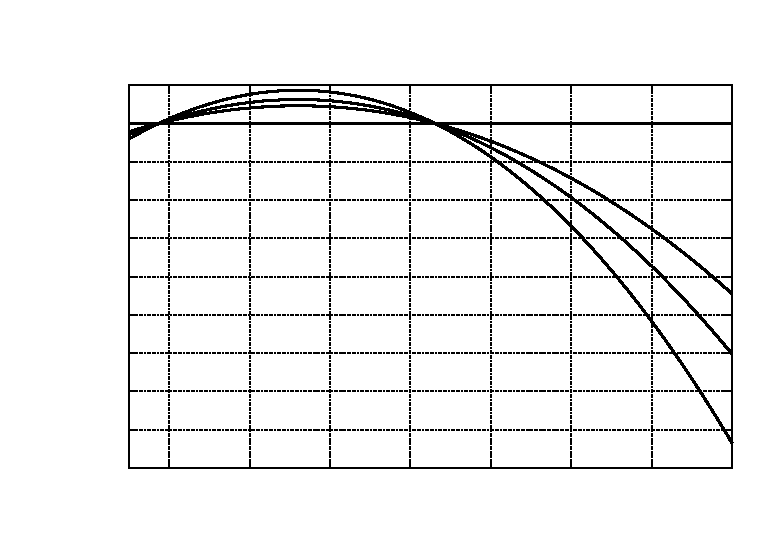
\includegraphics{../graphs/alt_error_flaps_up}}%
    \gplfronttext
  \end{picture}%
\endgroup
\end{center}  % for gnuplot epslatex, latex or pslatex mode
}
\caption{Position Error --- Altitude --- Flaps Retracted}
\label{SSEC-alt-error}
\end{figure}

               % Static Source Position Error, Altitude Chart
% ASI Instrument Error Chart
\begin{figure}[t]
% \addcontentsline{toc}{section}{Figure \ref{fg-asi-error} Airspeed Indicator Instrument Error}
\addcontentsline{toc}{section}{AIRSPEED INDICATOR INSTRUMENT ERROR}
%\addcontentsline{toc}{section}{Figure \ref{fg-asi-error} AIRSPEED INDICATOR INSTRUMENT ERROR}
\centering{
  \begin{perfhdr}AIRSPEED INDICATOR\\
  INSTRUMENT ERROR\\
  \end{perfhdr}
  % details of ASI
  \centering{\begin{minipage}{5in}\begin{tabbing}
  ASI Make - Model:aaaaa\= \kill
  ASI Make \& Model:\>UMA 16-311-241\\
  Serial \#:\>B0171\\
  Date of ground test:\>27 Apr 2004
  \end{tabbing}\end{minipage}}
  \begin{center}
  % GNUPLOT: LaTeX picture with Postscript
\begingroup
  \makeatletter
  \providecommand\color[2][]{%
    \GenericError{(gnuplot) \space\space\space\@spaces}{%
      Package color not loaded in conjunction with
      terminal option `colourtext'%
    }{See the gnuplot documentation for explanation.%
    }{Either use 'blacktext' in gnuplot or load the package
      color.sty in LaTeX.}%
    \renewcommand\color[2][]{}%
  }%
  \providecommand\includegraphics[2][]{%
    \GenericError{(gnuplot) \space\space\space\@spaces}{%
      Package graphicx or graphics not loaded%
    }{See the gnuplot documentation for explanation.%
    }{The gnuplot epslatex terminal needs graphicx.sty or graphics.sty.}%
    \renewcommand\includegraphics[2][]{}%
  }%
  \providecommand\rotatebox[2]{#2}%
  \@ifundefined{ifGPcolor}{%
    \newif\ifGPcolor
    \GPcolorfalse
  }{}%
  \@ifundefined{ifGPblacktext}{%
    \newif\ifGPblacktext
    \GPblacktexttrue
  }{}%
  % define a \g@addto@macro without @ in the name:
  \let\gplgaddtomacro\g@addto@macro
  % define empty templates for all commands taking text:
  \gdef\gplbacktext{}%
  \gdef\gplfronttext{}%
  \makeatother
  \ifGPblacktext
    % no textcolor at all
    \def\colorrgb#1{}%
    \def\colorgray#1{}%
  \else
    % gray or color?
    \ifGPcolor
      \def\colorrgb#1{\color[rgb]{#1}}%
      \def\colorgray#1{\color[gray]{#1}}%
      \expandafter\def\csname LTw\endcsname{\color{white}}%
      \expandafter\def\csname LTb\endcsname{\color{black}}%
      \expandafter\def\csname LTa\endcsname{\color{black}}%
      \expandafter\def\csname LT0\endcsname{\color[rgb]{1,0,0}}%
      \expandafter\def\csname LT1\endcsname{\color[rgb]{0,1,0}}%
      \expandafter\def\csname LT2\endcsname{\color[rgb]{0,0,1}}%
      \expandafter\def\csname LT3\endcsname{\color[rgb]{1,0,1}}%
      \expandafter\def\csname LT4\endcsname{\color[rgb]{0,1,1}}%
      \expandafter\def\csname LT5\endcsname{\color[rgb]{1,1,0}}%
      \expandafter\def\csname LT6\endcsname{\color[rgb]{0,0,0}}%
      \expandafter\def\csname LT7\endcsname{\color[rgb]{1,0.3,0}}%
      \expandafter\def\csname LT8\endcsname{\color[rgb]{0.5,0.5,0.5}}%
    \else
      % gray
      \def\colorrgb#1{\color{black}}%
      \def\colorgray#1{\color[gray]{#1}}%
      \expandafter\def\csname LTw\endcsname{\color{white}}%
      \expandafter\def\csname LTb\endcsname{\color{black}}%
      \expandafter\def\csname LTa\endcsname{\color{black}}%
      \expandafter\def\csname LT0\endcsname{\color{black}}%
      \expandafter\def\csname LT1\endcsname{\color{black}}%
      \expandafter\def\csname LT2\endcsname{\color{black}}%
      \expandafter\def\csname LT3\endcsname{\color{black}}%
      \expandafter\def\csname LT4\endcsname{\color{black}}%
      \expandafter\def\csname LT5\endcsname{\color{black}}%
      \expandafter\def\csname LT6\endcsname{\color{black}}%
      \expandafter\def\csname LT7\endcsname{\color{black}}%
      \expandafter\def\csname LT8\endcsname{\color{black}}%
    \fi
  \fi
  \setlength{\unitlength}{0.0500bp}%
  \begin{picture}(7200.00,5040.00)%
    \gplgaddtomacro\gplbacktext{%
      \csname LTb\endcsname%
      \put(814,704){\makebox(0,0)[r]{\strut{}-3}}%
      \csname LTb\endcsname%
      \put(814,1286){\makebox(0,0)[r]{\strut{}-2}}%
      \csname LTb\endcsname%
      \put(814,1867){\makebox(0,0)[r]{\strut{}-1}}%
      \csname LTb\endcsname%
      \put(814,2449){\makebox(0,0)[r]{\strut{} 0}}%
      \csname LTb\endcsname%
      \put(814,3030){\makebox(0,0)[r]{\strut{} 1}}%
      \csname LTb\endcsname%
      \put(814,3612){\makebox(0,0)[r]{\strut{} 2}}%
      \csname LTb\endcsname%
      \put(814,4193){\makebox(0,0)[r]{\strut{} 3}}%
      \csname LTb\endcsname%
      \put(814,4775){\makebox(0,0)[r]{\strut{} 4}}%
      \csname LTb\endcsname%
      \put(946,484){\makebox(0,0){\strut{} 0}}%
      \csname LTb\endcsname%
      \put(2131,484){\makebox(0,0){\strut{} 50}}%
      \csname LTb\endcsname%
      \put(3315,484){\makebox(0,0){\strut{} 100}}%
      \csname LTb\endcsname%
      \put(4500,484){\makebox(0,0){\strut{} 150}}%
      \csname LTb\endcsname%
      \put(5684,484){\makebox(0,0){\strut{} 200}}%
      \csname LTb\endcsname%
      \put(6869,484){\makebox(0,0){\strut{} 250}}%
      \put(308,2739){\rotatebox{-270}{\makebox(0,0){\strut{}ASI Instrument Error (kt)}}}%
      \put(3907,154){\makebox(0,0){\strut{}Airspeed Indicator Reading (kt)}}%
    }%
    \gplgaddtomacro\gplfronttext{%
      \put(3789,3903){\makebox(0,0){\strut{}ASI Reading = IAS + Error}}%
    }%
    \gplbacktext
    \put(0,0){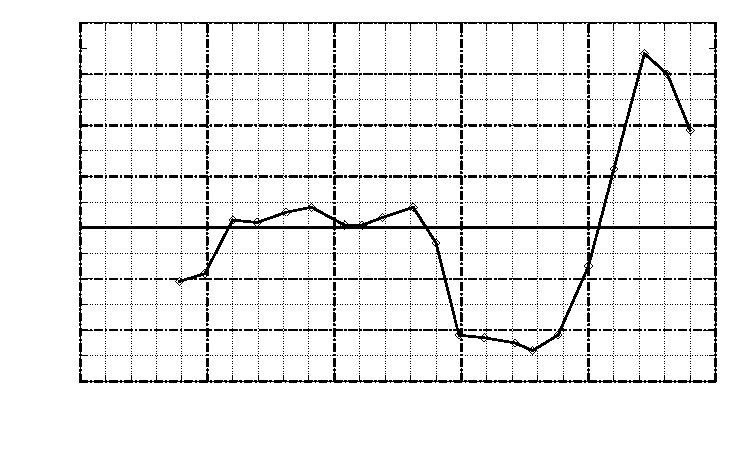
\includegraphics{../graphs/asi_error}}%
    \gplfronttext
  \end{picture}%
\endgroup

  \end{center}  % for gnuplot epslatex, latex or pslatex mode
}
\caption{Airspeed Indicator Instrument Error}
\label{fg-asi-error}
\end{figure}
%\lyxline{\normalsize}
%%%\vspace{0.1in}


         % ASI Instrument Error Chart
% EFIS Instrument Error Chart
%% try boxedminipage.sty to get box around figure, to help separate two figures if there are more than one per page
\begin{figure}[t]
% \addcontentsline{toc}{section}{Figure \ref{EFIS-asi-error} EFIS Airspeed Instrument Error}
\addcontentsline{toc}{section}{EFIS AIRSPEED INSTRUMENT ERROR}
\centering{
  \begin{perfhdr}EFIS AIRSPEED\\
  INSTRUMENT ERROR\\
  \end{perfhdr}
  % details of EFIS
  \centering{\begin{minipage}{5in}\begin{tabbing}
  EFIS Make - Model:aaaaa\= \kill
  EFIS Make \& Model:\>Dynon Development D-10A\\
  Part \#:\>100321- Rev 0\\
  Serial \#:\>004439\\
  Date of ground test:\>27 Apr 2004
  \end{tabbing}\end{minipage}}
  \begin{center}
  % GNUPLOT: LaTeX picture with Postscript
\begingroup
  \makeatletter
  \providecommand\color[2][]{%
    \GenericError{(gnuplot) \space\space\space\@spaces}{%
      Package color not loaded in conjunction with
      terminal option `colourtext'%
    }{See the gnuplot documentation for explanation.%
    }{Either use 'blacktext' in gnuplot or load the package
      color.sty in LaTeX.}%
    \renewcommand\color[2][]{}%
  }%
  \providecommand\includegraphics[2][]{%
    \GenericError{(gnuplot) \space\space\space\@spaces}{%
      Package graphicx or graphics not loaded%
    }{See the gnuplot documentation for explanation.%
    }{The gnuplot epslatex terminal needs graphicx.sty or graphics.sty.}%
    \renewcommand\includegraphics[2][]{}%
  }%
  \providecommand\rotatebox[2]{#2}%
  \@ifundefined{ifGPcolor}{%
    \newif\ifGPcolor
    \GPcolorfalse
  }{}%
  \@ifundefined{ifGPblacktext}{%
    \newif\ifGPblacktext
    \GPblacktexttrue
  }{}%
  % define a \g@addto@macro without @ in the name:
  \let\gplgaddtomacro\g@addto@macro
  % define empty templates for all commands taking text:
  \gdef\gplbacktext{}%
  \gdef\gplfronttext{}%
  \makeatother
  \ifGPblacktext
    % no textcolor at all
    \def\colorrgb#1{}%
    \def\colorgray#1{}%
  \else
    % gray or color?
    \ifGPcolor
      \def\colorrgb#1{\color[rgb]{#1}}%
      \def\colorgray#1{\color[gray]{#1}}%
      \expandafter\def\csname LTw\endcsname{\color{white}}%
      \expandafter\def\csname LTb\endcsname{\color{black}}%
      \expandafter\def\csname LTa\endcsname{\color{black}}%
      \expandafter\def\csname LT0\endcsname{\color[rgb]{1,0,0}}%
      \expandafter\def\csname LT1\endcsname{\color[rgb]{0,1,0}}%
      \expandafter\def\csname LT2\endcsname{\color[rgb]{0,0,1}}%
      \expandafter\def\csname LT3\endcsname{\color[rgb]{1,0,1}}%
      \expandafter\def\csname LT4\endcsname{\color[rgb]{0,1,1}}%
      \expandafter\def\csname LT5\endcsname{\color[rgb]{1,1,0}}%
      \expandafter\def\csname LT6\endcsname{\color[rgb]{0,0,0}}%
      \expandafter\def\csname LT7\endcsname{\color[rgb]{1,0.3,0}}%
      \expandafter\def\csname LT8\endcsname{\color[rgb]{0.5,0.5,0.5}}%
    \else
      % gray
      \def\colorrgb#1{\color{black}}%
      \def\colorgray#1{\color[gray]{#1}}%
      \expandafter\def\csname LTw\endcsname{\color{white}}%
      \expandafter\def\csname LTb\endcsname{\color{black}}%
      \expandafter\def\csname LTa\endcsname{\color{black}}%
      \expandafter\def\csname LT0\endcsname{\color{black}}%
      \expandafter\def\csname LT1\endcsname{\color{black}}%
      \expandafter\def\csname LT2\endcsname{\color{black}}%
      \expandafter\def\csname LT3\endcsname{\color{black}}%
      \expandafter\def\csname LT4\endcsname{\color{black}}%
      \expandafter\def\csname LT5\endcsname{\color{black}}%
      \expandafter\def\csname LT6\endcsname{\color{black}}%
      \expandafter\def\csname LT7\endcsname{\color{black}}%
      \expandafter\def\csname LT8\endcsname{\color{black}}%
    \fi
  \fi
  \setlength{\unitlength}{0.0500bp}%
  \begin{picture}(7200.00,5040.00)%
    \gplgaddtomacro\gplbacktext{%
      \csname LTb\endcsname%
      \put(814,704){\makebox(0,0)[r]{\strut{}-3}}%
      \csname LTb\endcsname%
      \put(814,1722){\makebox(0,0)[r]{\strut{}-2}}%
      \csname LTb\endcsname%
      \put(814,2740){\makebox(0,0)[r]{\strut{}-1}}%
      \csname LTb\endcsname%
      \put(814,3757){\makebox(0,0)[r]{\strut{} 0}}%
      \csname LTb\endcsname%
      \put(814,4775){\makebox(0,0)[r]{\strut{} 1}}%
      \csname LTb\endcsname%
      \put(946,484){\makebox(0,0){\strut{} 0}}%
      \csname LTb\endcsname%
      \put(2131,484){\makebox(0,0){\strut{} 50}}%
      \csname LTb\endcsname%
      \put(3315,484){\makebox(0,0){\strut{} 100}}%
      \csname LTb\endcsname%
      \put(4500,484){\makebox(0,0){\strut{} 150}}%
      \csname LTb\endcsname%
      \put(5684,484){\makebox(0,0){\strut{} 200}}%
      \csname LTb\endcsname%
      \put(6869,484){\makebox(0,0){\strut{} 250}}%
      \put(308,2739){\rotatebox{-270}{\makebox(0,0){\strut{}EFIS ASI Instrument Error (kt)}}}%
      \put(3907,154){\makebox(0,0){\strut{}EFIS Airspeed Reading (kt)}}%
    }%
    \gplgaddtomacro\gplfronttext{%
      \put(3789,1213){\makebox(0,0){\strut{}EFIS Airspeed Reading = IAS + Error}}%
    }%
    \gplbacktext
    \put(0,0){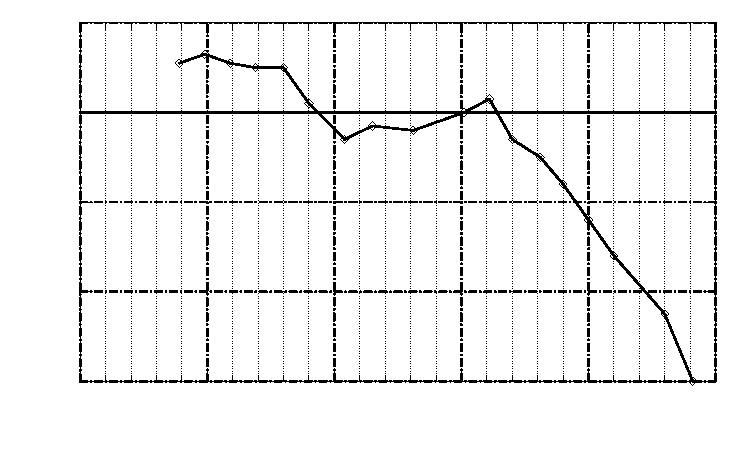
\includegraphics{../graphs/efis_error}}%
    \gplfronttext
  \end{picture}%
\endgroup
\end{center}  % for gnuplot epslatex, latex or pslatex mode
}
\caption{EFIS Airspeed Instrument Error}
\label{EFIS-asi-error}
\end{figure}


    % EFIS Instrument Error Chart
% EFIS Airspeed Error Chart --- Static Source Position Error + EFIS ASI instrument error
%% try boxedminipage.sty to get box around figure, to help separate two figures if there are more than one per page
\begin{figure}[t]
% \addcontentsline{toc}{section}{Figure \ref{EFIS-spd-error} EFIS Airspeed Error --- Airspeed --- Flaps Retracted}
\addcontentsline{toc}{section}{EFIS AIRSPEED ERROR --- AIRSPEED --- FLAPS RETRACTED}
\centering{
  \begin{perfhdr}EFIS AIRSPEED ERROR\\
  FLAPS RETRACTED\\
  \end{perfhdr}

  \centering{\begin{minipage}{5in}\begin{tabbing}
  EFIS Make --- Model:aaaaa\= \kill
  EFIS Make \& Model:\>Dynon Development D-10A\\
  Part \#:\>100321- Rev 0\\
  Serial \#:\>004439\\
  Date of ground test:\>27 Apr 2004\\
  \\
  Weight:\>1400 lb\\
  Flaps:\>Retracted\\
  Date of flight tests:\>14 \& 19 Nov 2008
  \end{tabbing}\end{minipage}}
  \begin{center}
  % GNUPLOT: LaTeX picture with Postscript
\begingroup
  \makeatletter
  \providecommand\color[2][]{%
    \GenericError{(gnuplot) \space\space\space\@spaces}{%
      Package color not loaded in conjunction with
      terminal option `colourtext'%
    }{See the gnuplot documentation for explanation.%
    }{Either use 'blacktext' in gnuplot or load the package
      color.sty in LaTeX.}%
    \renewcommand\color[2][]{}%
  }%
  \providecommand\includegraphics[2][]{%
    \GenericError{(gnuplot) \space\space\space\@spaces}{%
      Package graphicx or graphics not loaded%
    }{See the gnuplot documentation for explanation.%
    }{The gnuplot epslatex terminal needs graphicx.sty or graphics.sty.}%
    \renewcommand\includegraphics[2][]{}%
  }%
  \providecommand\rotatebox[2]{#2}%
  \@ifundefined{ifGPcolor}{%
    \newif\ifGPcolor
    \GPcolorfalse
  }{}%
  \@ifundefined{ifGPblacktext}{%
    \newif\ifGPblacktext
    \GPblacktexttrue
  }{}%
  % define a \g@addto@macro without @ in the name:
  \let\gplgaddtomacro\g@addto@macro
  % define empty templates for all commands taking text:
  \gdef\gplbacktext{}%
  \gdef\gplfronttext{}%
  \makeatother
  \ifGPblacktext
    % no textcolor at all
    \def\colorrgb#1{}%
    \def\colorgray#1{}%
  \else
    % gray or color?
    \ifGPcolor
      \def\colorrgb#1{\color[rgb]{#1}}%
      \def\colorgray#1{\color[gray]{#1}}%
      \expandafter\def\csname LTw\endcsname{\color{white}}%
      \expandafter\def\csname LTb\endcsname{\color{black}}%
      \expandafter\def\csname LTa\endcsname{\color{black}}%
      \expandafter\def\csname LT0\endcsname{\color[rgb]{1,0,0}}%
      \expandafter\def\csname LT1\endcsname{\color[rgb]{0,1,0}}%
      \expandafter\def\csname LT2\endcsname{\color[rgb]{0,0,1}}%
      \expandafter\def\csname LT3\endcsname{\color[rgb]{1,0,1}}%
      \expandafter\def\csname LT4\endcsname{\color[rgb]{0,1,1}}%
      \expandafter\def\csname LT5\endcsname{\color[rgb]{1,1,0}}%
      \expandafter\def\csname LT6\endcsname{\color[rgb]{0,0,0}}%
      \expandafter\def\csname LT7\endcsname{\color[rgb]{1,0.3,0}}%
      \expandafter\def\csname LT8\endcsname{\color[rgb]{0.5,0.5,0.5}}%
    \else
      % gray
      \def\colorrgb#1{\color{black}}%
      \def\colorgray#1{\color[gray]{#1}}%
      \expandafter\def\csname LTw\endcsname{\color{white}}%
      \expandafter\def\csname LTb\endcsname{\color{black}}%
      \expandafter\def\csname LTa\endcsname{\color{black}}%
      \expandafter\def\csname LT0\endcsname{\color{black}}%
      \expandafter\def\csname LT1\endcsname{\color{black}}%
      \expandafter\def\csname LT2\endcsname{\color{black}}%
      \expandafter\def\csname LT3\endcsname{\color{black}}%
      \expandafter\def\csname LT4\endcsname{\color{black}}%
      \expandafter\def\csname LT5\endcsname{\color{black}}%
      \expandafter\def\csname LT6\endcsname{\color{black}}%
      \expandafter\def\csname LT7\endcsname{\color{black}}%
      \expandafter\def\csname LT8\endcsname{\color{black}}%
    \fi
  \fi
  \setlength{\unitlength}{0.0500bp}%
  \begin{picture}(7200.00,5040.00)%
    \gplgaddtomacro\gplbacktext{%
      \csname LTb\endcsname%
      \put(814,704){\makebox(0,0)[r]{\strut{}-7}}%
      \csname LTb\endcsname%
      \put(814,1112){\makebox(0,0)[r]{\strut{}-6}}%
      \csname LTb\endcsname%
      \put(814,1521){\makebox(0,0)[r]{\strut{}-5}}%
      \csname LTb\endcsname%
      \put(814,1929){\makebox(0,0)[r]{\strut{}-4}}%
      \csname LTb\endcsname%
      \put(814,2337){\makebox(0,0)[r]{\strut{}-3}}%
      \csname LTb\endcsname%
      \put(814,2746){\makebox(0,0)[r]{\strut{}-2}}%
      \csname LTb\endcsname%
      \put(814,3154){\makebox(0,0)[r]{\strut{}-1}}%
      \csname LTb\endcsname%
      \put(814,3562){\makebox(0,0)[r]{\strut{} 0}}%
      \csname LTb\endcsname%
      \put(814,3971){\makebox(0,0)[r]{\strut{} 1}}%
      \csname LTb\endcsname%
      \put(814,4379){\makebox(0,0)[r]{\strut{} 2}}%
      \csname LTb\endcsname%
      \put(1258,484){\makebox(0,0){\strut{} 60}}%
      \csname LTb\endcsname%
      \put(1881,484){\makebox(0,0){\strut{} 80}}%
      \csname LTb\endcsname%
      \put(2505,484){\makebox(0,0){\strut{} 100}}%
      \csname LTb\endcsname%
      \put(3128,484){\makebox(0,0){\strut{} 120}}%
      \csname LTb\endcsname%
      \put(3752,484){\makebox(0,0){\strut{} 140}}%
      \csname LTb\endcsname%
      \put(4375,484){\makebox(0,0){\strut{} 160}}%
      \csname LTb\endcsname%
      \put(4999,484){\makebox(0,0){\strut{} 180}}%
      \csname LTb\endcsname%
      \put(5622,484){\makebox(0,0){\strut{} 200}}%
      \csname LTb\endcsname%
      \put(6246,484){\makebox(0,0){\strut{} 220}}%
      \csname LTb\endcsname%
      \put(6869,484){\makebox(0,0){\strut{} 240}}%
      \put(308,2541){\rotatebox{-270}{\makebox(0,0){\strut{}Error in Airspeed (kt)}}}%
      \put(3907,154){\makebox(0,0){\strut{}EFIS ASI Indication (kt)}}%
      \put(3907,4709){\makebox(0,0){\strut{}EFIS Airspeed Error - Flaps Retracted}}%
    }%
    \gplgaddtomacro\gplfronttext{%
      \put(3284,1725){\makebox(0,0){\strut{}CAS = EFIS ASI Indication + Error}}%
      \put(3284,1317){\makebox(0,0){\strut{}Chart Includes EFIS ASI Instrument Error}}%
    }%
    \gplbacktext
    \put(0,0){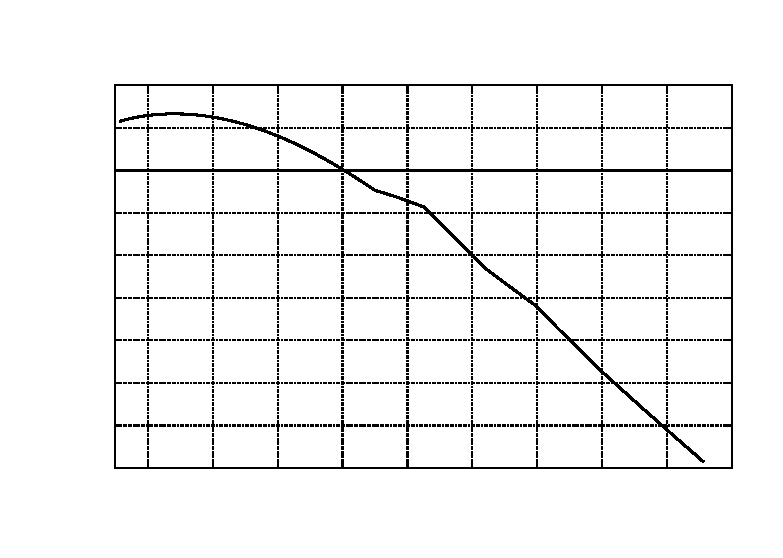
\includegraphics{../graphs/efis_ias_err_flaps_up}}%
    \gplfronttext
  \end{picture}%
\endgroup
\end{center}  % for gnuplot epslatex, latex or pslatex mode
}
\caption{EFIS Airspeed Error --- Airspeed --- Flaps Retracted}
\label{EFIS-spd-error}
\end{figure}


    % EFIS Airspeed Error Chart --- Static Source Position Error + EFIS ASI inst error
% EFIS ASI TAS Correction Table
\begin{figure}[t]
% \addcontentsline{toc}{section}{Figure \ref{TO-Dist} Takeoff Distance}
\addcontentsline{toc}{section}{EFIS ASI TAS CORRECTION}
\begin{center}
\begin{perfhdr}EFIS ASI TAS CORRECTION\\
1800 LBS
\end{perfhdr}
\Large
% \textcolor{red}{VANS CLAIMED PERF EXPANDED TO OTHER CONDITIONS}\vspace{1ex}\\
% \textcolor{red}{TO BE CONFIRMED BY FLIGHT TEST}\normalsize \vspace{5ex}\\

% \begin{minipage}{7.5in}
%   \begin{flushleft}
%     CONDITIONS:\\
%     Flaps 17\textdegree \ (set flap angle to match down aileron angle at full aileron)\\
%     2700 RPM, Full Throttle and Mixture Set prior to Brake Release\\
%     Paved, Level, Dry Runway\\
%     Zero Wind\\
% \vspace{\perfnoteskip}
%     NOTES:
%     \begin{enumerate*}
%       \item Short field technique as specified in Section \textcolor{red}{4}.
% %      \item Prior to takeoff from fields above 8,000 ft elevation, the mixture should be leaned to give maximum power in
% %      a full throttle static runup.
%       \item Set mixture at placard fuel flow.
%       \item Decrease distance by 10\% for each \textcolor{red}{X} knots headwind.  For operations with tailwinds up to 10
%       knots, increase distances by \textcolor{red}{10\%}.
%       \item For operation on a dry, grass runway, increase distances by \textcolor{red}{10\%} of the ground roll figure.
%       \end{enumerate*}
%     \end{flushleft}
%   \end{minipage}
% \hfill
% \begin{minipage}{1.5in}
%   \begin{tabular}{|c|c|}
%     \hline
%     \multicolumn{2}{|c|}{MIXTURE SETTING}\\
%     \hline
%     PRESS ALT&GPH\\
%     \hline
%     S.L.&17\\
%     2000&16\\
%     4000&15\\
%     6000&14\\
%     8000&13\\
%     \hline
%     \end{tabular}
%   \end{minipage}
% \\
\vspace{\perfnoteskip}
    \raggedright NOTES:
    \begin{enumerate*}
      \item Table provides TAS correction as a function of altitude and IAS.
      \item Corrected TAS = TAS displayed on EFIS + correction.
      \item Table includes static source position error, EFIS ASI instrument error and OAT ram temperature rise.
      \end{enumerate*}

\vspace{\perfnoteskip}
\settowidth{\colOne}{ALTITUDE}
% \settowidth{\colFive}{GRND}
\begin{tabular}{|c|c|c|c|c|c|c|c|c|c|c|c|}
\hline
\multirow{2}{\colOne}{\centering ALTITUDE (FT)}&\multicolumn{11}{c|}{IAS (KT)}\\
\cline{2-12}
&80&90&100&110&120&130&140&150&160&170&180\\
\hline
\hline
0&+1.2&+1.0&+0.8&+0.4&+0.0&-0.5&-0.7&-1.3&-2.1&-2.9&-3.6\\
\hline
5,000&+1.3&+1.1&+0.8&+0.4&-0.0&-0.6&-0.9&-1.5&-2.4&-3.2&-4.0\\
\hline
10,000&+1.3&+1.1&+0.8&+0.4&-0.1&-0.7&-1.0&-1.7&-2.7&-3.6&-4.5\\
\hline
15,000&+1.4&+1.2&+0.9&+0.4&-0.2&-0.8&-1.3&-2.0&-3.1&-4.2&-5.1\\
\hline
20,000&+1.5&+1.3&+0.9&+0.3&-0.3&-1.1&-1.5&-2.4&-3.6&-4.8&-5.8\\
\hline
&\multicolumn{11}{c|}{TAS CORRECTION (KT)}\\
\hline
\end{tabular}
\end{center}
\caption{EFIS ASI TAS Correction}
\label{EFIS-ASI-TAS-Corr}
\end{figure}

      % EFIS ASI TAS Correction Table
% Stall Speed Chart
\begin{figure}[t]
% \addcontentsline{toc}{section}{Figure \ref{stall-speed-kcas} Stall Speed --- KCAS}
\addcontentsline{toc}{section}{STALL SPEED --- KCAS}
\begin{center}
\begin{perfhdr}STALL SPEED --- KCAS\\
\end{perfhdr}

\begin{minipage}{2in}
  \begin{flushleft}
    CONDITIONS:\\
    Idle power\\
    Prop control at Max RPM\\
    Deceleration at 1 kt/s\\
    \end{flushleft}
  \end{minipage}\\
%\vspace{2ex}
% GNUPLOT: LaTeX picture with Postscript
\begingroup
  \makeatletter
  \providecommand\color[2][]{%
    \GenericError{(gnuplot) \space\space\space\@spaces}{%
      Package color not loaded in conjunction with
      terminal option `colourtext'%
    }{See the gnuplot documentation for explanation.%
    }{Either use 'blacktext' in gnuplot or load the package
      color.sty in LaTeX.}%
    \renewcommand\color[2][]{}%
  }%
  \providecommand\includegraphics[2][]{%
    \GenericError{(gnuplot) \space\space\space\@spaces}{%
      Package graphicx or graphics not loaded%
    }{See the gnuplot documentation for explanation.%
    }{The gnuplot epslatex terminal needs graphicx.sty or graphics.sty.}%
    \renewcommand\includegraphics[2][]{}%
  }%
  \providecommand\rotatebox[2]{#2}%
  \@ifundefined{ifGPcolor}{%
    \newif\ifGPcolor
    \GPcolorfalse
  }{}%
  \@ifundefined{ifGPblacktext}{%
    \newif\ifGPblacktext
    \GPblacktexttrue
  }{}%
  % define a \g@addto@macro without @ in the name:
  \let\gplgaddtomacro\g@addto@macro
  % define empty templates for all commands taking text:
  \gdef\gplbacktext{}%
  \gdef\gplfronttext{}%
  \makeatother
  \ifGPblacktext
    % no textcolor at all
    \def\colorrgb#1{}%
    \def\colorgray#1{}%
  \else
    % gray or color?
    \ifGPcolor
      \def\colorrgb#1{\color[rgb]{#1}}%
      \def\colorgray#1{\color[gray]{#1}}%
      \expandafter\def\csname LTw\endcsname{\color{white}}%
      \expandafter\def\csname LTb\endcsname{\color{black}}%
      \expandafter\def\csname LTa\endcsname{\color{black}}%
      \expandafter\def\csname LT0\endcsname{\color[rgb]{1,0,0}}%
      \expandafter\def\csname LT1\endcsname{\color[rgb]{0,1,0}}%
      \expandafter\def\csname LT2\endcsname{\color[rgb]{0,0,1}}%
      \expandafter\def\csname LT3\endcsname{\color[rgb]{1,0,1}}%
      \expandafter\def\csname LT4\endcsname{\color[rgb]{0,1,1}}%
      \expandafter\def\csname LT5\endcsname{\color[rgb]{1,1,0}}%
      \expandafter\def\csname LT6\endcsname{\color[rgb]{0,0,0}}%
      \expandafter\def\csname LT7\endcsname{\color[rgb]{1,0.3,0}}%
      \expandafter\def\csname LT8\endcsname{\color[rgb]{0.5,0.5,0.5}}%
    \else
      % gray
      \def\colorrgb#1{\color{black}}%
      \def\colorgray#1{\color[gray]{#1}}%
      \expandafter\def\csname LTw\endcsname{\color{white}}%
      \expandafter\def\csname LTb\endcsname{\color{black}}%
      \expandafter\def\csname LTa\endcsname{\color{black}}%
      \expandafter\def\csname LT0\endcsname{\color{black}}%
      \expandafter\def\csname LT1\endcsname{\color{black}}%
      \expandafter\def\csname LT2\endcsname{\color{black}}%
      \expandafter\def\csname LT3\endcsname{\color{black}}%
      \expandafter\def\csname LT4\endcsname{\color{black}}%
      \expandafter\def\csname LT5\endcsname{\color{black}}%
      \expandafter\def\csname LT6\endcsname{\color{black}}%
      \expandafter\def\csname LT7\endcsname{\color{black}}%
      \expandafter\def\csname LT8\endcsname{\color{black}}%
    \fi
  \fi
  \setlength{\unitlength}{0.0500bp}%
  \begin{picture}(7200.00,5040.00)%
    \gplgaddtomacro\gplbacktext{%
      \csname LTb\endcsname%
      \put(1078,704){\makebox(0,0)[r]{\strut{} 1300}}%
      \csname LTb\endcsname%
      \put(1078,1383){\makebox(0,0)[r]{\strut{} 1400}}%
      \csname LTb\endcsname%
      \put(1078,2061){\makebox(0,0)[r]{\strut{} 1500}}%
      \csname LTb\endcsname%
      \put(1078,2740){\makebox(0,0)[r]{\strut{} 1600}}%
      \csname LTb\endcsname%
      \put(1078,3418){\makebox(0,0)[r]{\strut{} 1700}}%
      \csname LTb\endcsname%
      \put(1078,4097){\makebox(0,0)[r]{\strut{} 1800}}%
      \csname LTb\endcsname%
      \put(1078,4775){\makebox(0,0)[r]{\strut{} 1900}}%
      \csname LTb\endcsname%
      \put(1210,484){\makebox(0,0){\strut{} 45}}%
      \csname LTb\endcsname%
      \put(2608,484){\makebox(0,0){\strut{} 50}}%
      \csname LTb\endcsname%
      \put(4007,484){\makebox(0,0){\strut{} 55}}%
      \csname LTb\endcsname%
      \put(5405,484){\makebox(0,0){\strut{} 60}}%
      \csname LTb\endcsname%
      \put(6803,484){\makebox(0,0){\strut{} 65}}%
      \put(176,2739){\rotatebox{-270}{\makebox(0,0){\strut{}Gross Weight (lb)}}}%
      \put(4006,154){\makebox(0,0){\strut{}Stall Speed (KCAS)}}%
      \put(3028,2740){\rotatebox{57}{\makebox(0,0)[l]{\strut{}Full Flap}}}%
      \put(4146,2061){\rotatebox{52}{\makebox(0,0)[l]{\strut{}Flaps UP}}}%
    }%
    \gplgaddtomacro\gplfronttext{%
    }%
    \gplbacktext
    \put(0,0){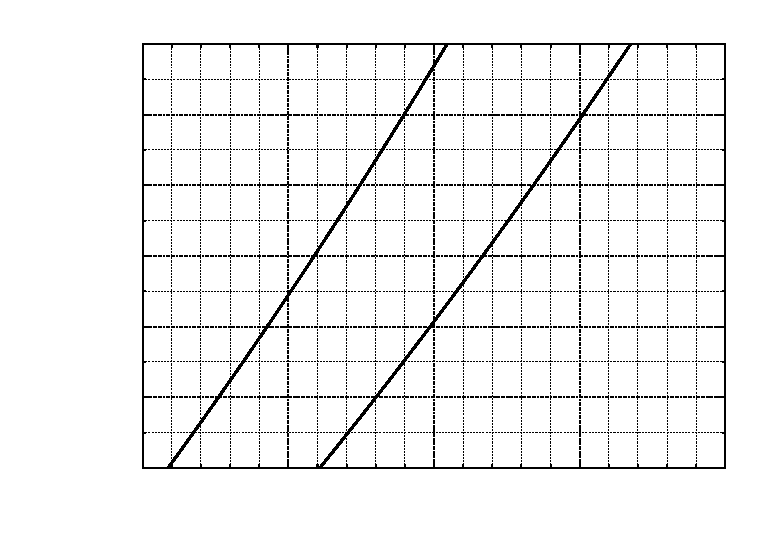
\includegraphics{../graphs/stall}}%
    \gplfronttext
  \end{picture}%
\endgroup
\end{center}  % for gnuplot epslatex, latex or pslatex mode
\caption{Stall Speed --- KCAS}
\label{stall-speed-kcas}
\end{figure}
\clearpage


            % Stall Speed Chart
% Takeoff Performance
\begin{sidewaysfigure}[t]
% \addcontentsline{toc}{section}{Figure \ref{TO-Dist} Takeoff Distance}
\addcontentsline{toc}{section}{TAKEOFF DISTANCE}
\begin{center}
\begin{perfhdr}TAKEOFF DISTANCE\\
1800 LBS
\end{perfhdr}
\Large
\textcolor{red}{VANS CLAIMED PERF EXPANDED TO OTHER CONDITIONS}\vspace{1ex}\\
\textcolor{red}{TO BE CONFIRMED BY FLIGHT TEST}\normalsize \vspace{5ex}\\

\begin{minipage}{7.5in}
  \begin{flushleft}
    CONDITIONS:\\
    Flaps 17\textdegree \ (set flap angle to match down aileron angle at full aileron)\\
    2700 RPM, Full Throttle and Mixture Set prior to Brake Release\\
    Paved, Level, Dry Runway\\
    Zero Wind\\
\vspace{\perfnoteskip}
    NOTES:
    \begin{enumerate*}
      \item Short field technique as specified in Section \textcolor{red}{4}.
%      \item Prior to takeoff from fields above 8,000 ft elevation, the mixture should be leaned to give maximum power in
%      a full throttle static runup.
      \item Set mixture at placard fuel flow.
      \item Decrease distance by 10\% for each \textcolor{red}{X} knots headwind.  For operations with tailwinds up to 10
      knots, increase distances by \textcolor{red}{10\%}.
      \item For operation on a dry, grass runway, increase distances by \textcolor{red}{10\%} of the ground roll figure.
      \end{enumerate*}
    \end{flushleft}
  \end{minipage}
\hfill
\begin{minipage}{1.5in}
  \begin{tabular}{|c|c|}
    \hline
    \multicolumn{2}{|c|}{MIXTURE SETTING}\\
    \hline
    PRESS ALT&GPH\\
    \hline
    S.L.&17\\
    2000&16\\
    4000&15\\
    6000&14\\
    8000&13\\
    \hline
    \end{tabular}
  \end{minipage}
\\

\vspace{\perfnoteskip}
\settowidth{\colOne}{WEIGHT}
\settowidth{\colFive}{GRND}
\begin{tabular}{|c|c|c|r|r|r|r|r|r|r|r|r|r|r|}
\hline
\multirow{5}{\colOne}{\centering WEIGHT (LB)}&\multicolumn{2}{c|}{TAKEOFF}&&\multicolumn{2}{c|}{0\textdegree C}&\multicolumn{2}{c|}{10\textdegree C}&\multicolumn{2}{c|}{20\textdegree C}&\multicolumn{2}{c|}{30\textdegree C}&\multicolumn{2}{c|}{40\textdegree C}\\
\cline{5-14}
&\multicolumn{2}{c|}{SPEED}&\multicolumn{1}{c|}{PRESS}&\multirow{4}{\colFive}{\centering GRND ROLL (FT)}&
\multicolumn{1}{c|}{TOTAL}&\multirow{4}{\colFive}{\centering GRND ROLL (FT)}&
\multicolumn{1}{c|}{TOTAL}&\multirow{4}{\colFive}{\centering GRND ROLL (FT)}&
\multicolumn{1}{c|}{TOTAL}&\multirow{4}{\colFive}{\centering GRND ROLL (FT)}&
\multicolumn{1}{c|}{TOTAL}&\multirow{4}{\colFive}{\centering GRND ROLL (FT)}&\multicolumn{1}{c|}{TOTAL}\\
&\multicolumn{2}{c|}{(KIAS)}&\multicolumn{1}{c|}{ALT}&&\multicolumn{1}{c|}{DIST}&&
\multicolumn{1}{c|}{DIST}&&\multicolumn{1}{c|}{DIST}&&\multicolumn{1}{c|}{DIST}&&\multicolumn{1}{c|}{DIST}\\
\cline{2-3}
&LIFT&AT&\multicolumn{1}{c|}{(FT)}&&\multicolumn{1}{c|}{TO}&&\multicolumn{1}{c|}{TO}&&
\multicolumn{1}{c|}{TO}&&\multicolumn{1}{c|}{TO}&&\multicolumn{1}{c|}{TO}\\
&OFF&50 FT&&&\multicolumn{1}{c|}{50 FT}&&\multicolumn{1}{c|}{50 FT}&&\multicolumn{1}{c|}{50 FT}&&\multicolumn{1}{c|}{50 FT}&&\multicolumn{1}{c|}{50 FT}\\
\hline
\hline

1800&XX&YY&S.L.&460&TTT&490&TTT&510&TTT&550&TTT&580&TTT\\
\hline
&XX&YY&2,000&550&TTT&590&TTT&620&TTT&660&TTT&700&TTT\\
\hline
&XX&YY&4,000&670&TTT&710&TTT&750&TTT&800&TTT&840&TTT\\
\hline
&XX&YY&6,000&810&TTT&860&TTT&920&TTT&970&TTT&1020&TTT\\
\hline
&XX&YY&8,000&990&TTT&1050&TTT&1120&TTT&1180&TTT&1250&TTT\\
\hline
&XX&YY&10,000&1210&TTT&1280&TTT&1360&TTT&1440&TTT&1520&TTT\\
\hline
&XX&YY&12,000&1480&TTT&1570&TTT&1670&TTT&1770&TTT&1870&TTT\\
\hline
\end{tabular}
\end{center}
\caption{Takeoff Distance}
\label{TO-Dist}
\end{sidewaysfigure}

                % Takeoff Performance
% Rate of Climb Chart
\begin{figure}[t]
% \addcontentsline{toc}{section}{Figure \ref{ROC-Max} Rate of Climb --- Maximum Power}
\addcontentsline{toc}{section}{RATE OF CLIMB --- MAXIMUM POWER}
\begin{center}
\begin{perfhdr}RATE OF CLIMB
\end{perfhdr}
\Large
% \textcolor{red}{DATA TO BE CONFIRMED BY FLIGHT TEST}\normalsize \\
\vspace{5ex}
\begin{minipage}{4in}
  \begin{flushleft}
    CONDITIONS:\\
    Flaps UP\\
    2650 RPM\\
    Full Throttle\\
    Mixture Set to give EGT 25\textdegree F less than EGT during take-off\\
%    NOTE:
%    Mixture leaned when power is at 75\% power or less (8,000 ft or above at standard temperature) for smooth
%    engine operation and increased power.
    \end{flushleft}
  \end{minipage}
\hfill
% \begin{minipage}{1.5in}
%   \begin{tabular}{|c|c|}
%     \hline
%     \multicolumn{2}{|c|}{MIXTURE SETTING}\\
%     \hline
%     PRESS ALT&GPH\\
%     \hline
%     S.L.&17\\
%     2000&16\\
%     4000&15\\
%     6000&14\\
%     8000&13\\
%     \hline
%     \end{tabular}
%   \end{minipage}
\\
\vspace{\perfnoteskip}

\settowidth{\colOne}{WEIGHT}
\settowidth{\colTwo}{PRESSURE}
\settowidth{\colThree}{CLIMB}
\settowidth{\colFour}{-20\textdegree C}
\settowidth{\colFive}{9,999}
\settowidth{\colSix}{9,999}
\settowidth{\colSeven}{9,999}

\begin{tabular}{|c|r|r|r|r|r|r|}
\hline
\multirow{3}{\colOne}{\centering WEIGHT (LB)}&\multirow{3}{\colTwo}{\centering PRESSURE ALTITUDE (FT)}&
\multirow{3}{\colThree}{\centering CLIMB SPEED (KIAS)}&
\multicolumn{4}{c|}{RATE OF CLIMB (FT/MN)}\\
\cline{4-7}
&&&\multirow{2}{\colFour}{\centering -20\textdegree C}&\multirow{2}{\colFive}{\centering 0\textdegree C}&
\multirow{2}{\colSix}{\centering 20\textdegree C}&\multirow{2}{\colSeven}{\centering 40\textdegree C}\\
&&&&&&\\
\hline
\hline
% 1,800&0&102&2,090&1,930&1,770&1,600\\
% \hline
% 1,800&2,000&100&1,890&1,730&1,550&1,390\\
% \hline
% 1,800&4,000&98&1,720&1,530&1,360&1,210\\
% \hline
% 1,800&6,000&96&1,510&1,330&1,170&1,030\\
% \hline
% 1,800&8,000&94&1,290&1,120&970&840\\
% \hline
% 1,800&10,000&92&1,080&920&780&660\\
% \hline
% 1,800&12,000&90&880&730&590&480\\
% \hline
% 1,800&14,000&88&680&540&410&310\\
% \hline
% 1,800&16,000&86&480&350&240&140\\
% \hline
% 1,800&18,000&84&280&160&70&-20\\
% \hline
% 1,800&20,000&82&90&-10&-100&-180\\
% \hline
1,800&0&102&2,090&1,930&1,770&1,600\\
\hline
1,800&2,000&100&1,890&1,730&1,550&1,390\\
\hline
1,800&4,000&98&1,720&1,530&1,360&1,210\\
\hline
1,800&6,000&96&1,510&1,330&1,170&1,030\\
\hline
1,800&8,000&94&1,290&1,120&970&840\\
\hline
1,800&10,000&92&1,080&920&780&660\\
\hline
1,800&12,000&90&880&730&590&480\\
\hline
1,800&14,000&90&680&540&410&310\\
\hline
1,800&16,000&90&480&350&240&140\\
\hline
1,800&18,000&90&280&160&70&-20\\
\hline
1,800&20,000&90&90&-10&-100&-180\\
\hline
\end{tabular}
\end{center}
\caption{Rate of Climb --- Maximum Power}
\label{ROC-Max}
\end{figure}


      % Rate of Climb vs Temperature Chart
% Rate of Climb Chart
\begin{figure}[t]
% \addcontentsline{toc}{section}{Figure \ref{ROC-Max} Rate of Climb --- Maximum Power}
\addcontentsline{toc}{section}{RATE OF CLIMB --- MAXIMUM POWER --- 1900 lb}
\begin{center}
\begin{perfhdr}RATE OF CLIMB --- 1900 lb
\end{perfhdr}
% \Large
% \textcolor{red}{DATA TO BE CONFIRMED BY FLIGHT TEST}\normalsize \\
\vspace{5ex}
\begin{minipage}{4in}
  \begin{flushleft}
    CONDITIONS:\\
    1900 lb gross weight\\
    Flaps UP\\
    2650 RPM\\
    Full Throttle\\
    Mixture Set to give EGT 25\textdegree F less than EGT during take-off\\
%    NOTE:
%    Mixture leaned when power is at 75\% power or less (8,000 ft or above at standard temperature) for smooth
%    engine operation and increased power.
    \end{flushleft}
  \end{minipage}
\hfill
% \begin{minipage}{1.5in}
%   \begin{tabular}{|c|c|}
%     \hline
%     \multicolumn{2}{|c|}{MIXTURE SETTING}\\
%     \hline
%     PRESS ALT&GPH\\
%     \hline
%     S.L.&17\\
%     2000&16\\
%     4000&15\\
%     6000&14\\
%     8000&13\\
%     \hline
%     \end{tabular}
%   \end{minipage}
\\
\vspace{\perfnoteskip}

\settowidth{\colOne}{WEIGHT}
\settowidth{\colTwo}{PRESSURE}
\settowidth{\colThree}{CLIMB}
\settowidth{\colFour}{-20\textdegree C}
\settowidth{\colFive}{9,999}
\settowidth{\colSix}{9,999}
\settowidth{\colSeven}{9,999}

\begin{tabular}{|c|r|r|r|r|r|r|}
\hline
\multirow{3}{\colOne}{\centering WEIGHT (LB)}&\multirow{3}{\colTwo}{\centering PRESSURE ALTITUDE (FT)}&
\multirow{3}{\colThree}{\centering CLIMB SPEED (KIAS)}&
\multicolumn{4}{c|}{RATE OF CLIMB (FT/MN)}\\
\cline{4-7}
&&&\multirow{2}{\colFour}{\centering -20\textdegree C}&\multirow{2}{\colFive}{\centering 0\textdegree C}&
\multirow{2}{\colSix}{\centering 20\textdegree C}&\multirow{2}{\colSeven}{\centering 40\textdegree C}\\
&&&&&&\\
\hline
\hline
 % Data from Climb_DA_fit.py
1,900&0&102&1,930&1,780&1,630&1,470\\
\hline
1,900&2,000&100&1,740&1,590&1,420&1,270\\
\hline
1,900&4,000&98&1,580&1,400&1,240&1,100\\
\hline
1,900&6,000&96&1,380&1,210&1,060&930\\
\hline
1,900&8,000&94&1,170&1,010&870&750\\
\hline
1,900&10,000&92&970&820&690&570\\
\hline
1,900&12,000&90&770&630&510&400\\
\hline
1,900&14,000&90&580&450&330&240\\
\hline
1,900&16,000&90&390&270&170&80\\
\hline
1,900&18,000&90&200&90&0&-80\\
\hline
1,900&20,000&90&20&-80&-160&-230\\
\hline
\end{tabular}
\end{center}
\caption{Rate of Climb --- Maximum Power --- 1900 lb}
\label{ROC-Max}
\end{figure}


      % Rate of Climb vs Temperature Chart --- 1900 lb
% Time, Fuel and Distance to Climb table --- Max Power
\begin{figure}[t]
% \addcontentsline{toc}{section}{Figure \ref{TFD-to-climb-Max} Time, Fuel and Distance to Climb --- Maximum Power}
\addcontentsline{toc}{section}{TIME, FUEL AND DISTANCE TO CLIMB --- MAXIMUM POWER}
\begin{center}
\begin{perfhdr}TIME, FUEL AND DISTANCE TO CLIMB\\
MAXIMUM POWER\\
\end{perfhdr}
\Large
% \textcolor{red}{DATA TO BE CONFIRMED BY FLIGHT TEST}\\
\normalsize \vspace{5ex} 
\raggedright 
    CONDITIONS:\\
    Flaps UP\\
    2650 RPM\\
    Full Throttle\\
    Mixture Set to give EGT 25\textdegree F less than EGT during take-off\\
    Standard Temperature\\

\hfill

\vspace{\perfnoteskip}
    \raggedright NOTES:
    \begin{enumerate*}
      \item Add 1.0 USG of fuel for engine start, taxi and takeoff.
%      \item Mixture leaned when power is at 75\% power or less (8,000 ft or above at standard temperature) for smooth
%      engine operation and increased power.
      \item Climb speed is 102 KIAS at sea level, decreasing by 1 kt per 1000 ft.
      \item Increase time, fuel and distance by 10\% for each 10\textdegree C above standard
      temperatures.
      \item Distances shown are based on zero wind.
      \end{enumerate*}

\vspace{\perfnoteskip}
% following lengths are used to set row widths to fit the text
\settowidth{\colOne}{WEIGHT}
\settowidth{\colTwo}{PRESS.}
\settowidth{\colThree}{TEMP}
\settowidth{\colFour}{CLIMB}
\settowidth{\colFive}{RATE OF}
\settowidth{\colSix}{TIME}
\settowidth{\colSeven}{USED}
\settowidth{\colEight}{DIST.}

\begin{tabular}{|c|r|r|r|r|r|r|r|}
\hline
\multirow{3}{\colOne}[\halfrowdrop]{\centering WEIGHT (LB)}&\multirow{3}{\colTwo}[\halfrowdrop]{\centering PRESS. ALT. (FT)}&
\multirow{3}{\colThree}[\halfrowdrop]{\centering TEMP (\textdegree C)}&\multirow{3}{\colFour}[\halfrowdrop]{\centering CLIMB SPEED (KIAS)}&
\multirow{3}{\colFive}[\halfrowdrop]{\centering RATE OF CLIMB (FT/MN)}&\multicolumn{3}{c|}{FROM SEA LEVEL}\\
\cline{6-8}
&&&&&\multicolumn{1}{m{\colSix}|}{\centering TIME (MN)}&\multicolumn{1}{m{\colSeven}|}{\centering FUEL USED (USG)}&\multicolumn{1}{m{\colEight}|}{\centering DIST. (NM)}\\
\hline
\hline
% % START of copied data from python Climb_DA_fit.py script
% % Based on climb tests on flights 261, 262, 263 & 264
1,800&0&15&102&1,810&0&0&0\\
\hline
&2,000&11&100&1,640&1&0.3&2\\
\hline
&4,000&7&98&1,470&2&0.7&4\\
\hline
&6,000&3&96&1,300&4&1.0&7\\
\hline
&8,000&-1&94&1,130&6&1.4&10\\
\hline
&10,000&-5&92&960&7&1.8&13\\
\hline
&12,000&-9&90&790&10&2.3&17\\
\hline
&14,000&-13&90&620&13&2.9&22\\
\hline
&16,000&-17&90&450&16&3.5&29\\
\hline
&18,000&-21&90&290&22&4.5&40\\
\hline
&20,000&-25&90&120&32&6.1&60\\
\hline
% % END of copied data from python Climb_DA_fit.py script
\end{tabular}
\end{center}
\caption{Time, Fuel and Distance to Climb --- Maximum Power}
\label{TFD-to-climb-Max}
\end{figure}



         % Time, Fuel and Distance to Climb table --- Max Power
% Time, Fuel and Distance to Climb table --- Max Power
\begin{figure}[t]
% \addcontentsline{toc}{section}{Figure \ref{TFD-to-climb-Max} Time, Fuel and Distance to Climb --- Maximum Power}
\addcontentsline{toc}{section}{TIME, FUEL AND DISTANCE TO CLIMB --- MAXIMUM POWER --- 1900 lb}
\begin{center}
\begin{perfhdr}TIME, FUEL AND DISTANCE TO CLIMB --- 1900 lb\\
MAXIMUM POWER\\
\end{perfhdr}
\Large
% \textcolor{red}{DATA TO BE CONFIRMED BY FLIGHT TEST}\\
\normalsize \vspace{5ex} 
\raggedright 
    CONDITIONS:\\
    1900 lb gross weight\\
    Flaps UP\\
    2650 RPM\\
    Full Throttle\\
    Mixture Set to give EGT 25\textdegree F less than EGT during take-off\\
    Standard Temperature\\

\hfill

\vspace{\perfnoteskip}
    \raggedright NOTES:
    \begin{enumerate*}
      \item Add 1.0 USG of fuel for engine start, taxi and takeoff.
%      \item Mixture leaned when power is at 75\% power or less (8,000 ft or above at standard temperature) for smooth
%      engine operation and increased power.
      \item Climb speed is 102 KIAS at sea level, decreasing by 1 kt per 1000 ft.
      \item Increase time, fuel and distance by 10\% for each 10\textdegree C above standard
      temperatures.
      \item Distances shown are based on zero wind.
      \end{enumerate*}

\vspace{\perfnoteskip}
% following lengths are used to set row widths to fit the text
\settowidth{\colOne}{WEIGHT}
\settowidth{\colTwo}{PRESS.}
\settowidth{\colThree}{TEMP}
\settowidth{\colFour}{CLIMB}
\settowidth{\colFive}{RATE OF}
\settowidth{\colSix}{TIME}
\settowidth{\colSeven}{USED}
\settowidth{\colEight}{DIST.}

\begin{tabular}{|c|r|r|r|r|r|r|r|}
\hline
\multirow{3}{\colOne}[\halfrowdrop]{\centering WEIGHT (LB)}&\multirow{3}{\colTwo}[\halfrowdrop]{\centering PRESS. ALT. (FT)}&
\multirow{3}{\colThree}[\halfrowdrop]{\centering TEMP (\textdegree C)}&\multirow{3}{\colFour}[\halfrowdrop]{\centering CLIMB SPEED (KIAS)}&
\multirow{3}{\colFive}[\halfrowdrop]{\centering RATE OF CLIMB (FT/MN)}&\multicolumn{3}{c|}{FROM SEA LEVEL}\\
\cline{6-8}
&&&&&\multicolumn{1}{m{\colSix}|}{\centering TIME (MN)}&\multicolumn{1}{m{\colSeven}|}{\centering FUEL USED (USG)}&\multicolumn{1}{m{\colEight}|}{\centering DIST. (NM)}\\
\hline
\hline
% % START of copied data from python Climb_DA_fit.py script
% % Based on climb tests on flights 261, 262, 263 & 264
1,900&0&15&102&1,670&0&0&0\\
\hline
&2,000&11&100&1,510&1&0.4&2\\
\hline
&4,000&7&98&1,340&3&0.7&5\\
\hline
&6,000&3&96&1,180&4&1.1&7\\
\hline
&8,000&-1&94&1,020&6&1.6&11\\
\hline
&10,000&-5&92&850&8&2.0&14\\
\hline
&12,000&-9&90&690&11&2.6&19\\
\hline
&14,000&-13&90&530&14&3.2&25\\
\hline
&16,000&-17&90&360&19&4.0&33\\
\hline
&18,000&-21&90&200&26&5.2&47\\
\hline
&20,000&-25&90&40&43&7.9&81\\
\hline
% % END of copied data from python Climb_DA_fit.py script
\end{tabular}
\end{center}
\caption{Time, Fuel and Distance to Climb --- Maximum Power --- 1900 lb}
\label{TFD-to-climb-Max}
\end{figure}



         % Time, Fuel and Distance to Climb table --- Max Power --- 1900 lb
% % Time, Fuel and Distance to Climb table --- Normal Climb Power
\begin{figure}[t]
% \addcontentsline{toc}{section}{Figure \ref{TFD-to-climb-Norm} Time, Fuel and Distance to Climb --- Normal Climb Power}
\addcontentsline{toc}{section}{TIME, FUEL AND DISTANCE TO CLIMB --- NORMAL CLIMB POWER}
\begin{center}
\begin{perfhdr}TIME, FUEL AND DISTANCE TO CLIMB\\
NORMAL CLIMB\\
\end{perfhdr}
\Large
% \textcolor{red}{DATA TO BE CONFIRMED BY FLIGHT TEST}\\
\normalsize
\vspace{5ex}
\begin{minipage}{4in}
  \begin{flushleft}
    CONDITIONS:\\
    Flaps UP\\
    2650 RPM\\
    Full Throttle\\
    Mixture Set at Indicated Fuel Flow
    Standard Temperature\\
    \end{flushleft}
\end{minipage}
\hfill
\begin{minipage}{1.5in}
  \begin{tabular}{|c|c|}
    \hline
    \multicolumn{2}{|c|}{MIXTURE SETTING}\\
    \hline
    PRESS ALT&GPH\\
    \hline
    S.L.&17\\
    2000&16\\
    4000&15\\
    6000&14\\
    8000&13\\
    10,000&12.5\\
    12,000&11.8\\
    14,000&11.1\\
    16,000&10.4\\
    \hline
    \end{tabular}
  \end{minipage}
\\
\vspace{\perfnoteskip}
    \raggedright NOTES:
    \begin{enumerate*}
      \item Add 1.5 USG of fuel for engine start, taxi and takeoff.
%      \item Mixture leaned when power is at 75\% power or less (6,000 ft or above at standard temperature) for smooth engine operation and increased power.
      \item Climb speed is 100 KIAS from sea level to 10,000 ft, then decreasing by 2 kt per 1000 ft above 10,000 ft.
      \item Increase time, fuel and distance by \textcolor{red}{XX\%} for each 10\textdegree C above standard temperatures.
      \item Distances shown are based on zero wind.
      \end{enumerate*}
\vspace{\perfnoteskip}
% following lengths are used to set row widths to fit the text
\settowidth{\colOne}{WEIGHT}
\settowidth{\colTwo}{PRESSURE}
\settowidth{\colThree}{TEMP}
\settowidth{\colFour}{CLIMB}
\settowidth{\colFive}{RATE OF}
\settowidth{\colSix}{TIME}
\settowidth{\colSeven}{USED}
\settowidth{\colEight}{DIST.}

\begin{tabular}{|c|r|r|r|r|r|r|r|}
\hline
\multirow{3}{\colOne}[\halfrowdrop]{\centering WEIGHT (LB)}&\multirow{3}{\colTwo}[\halfrowdrop]{\centering PRESSURE ALTITUDE (FT)}&
\multirow{3}{\colThree}[\halfrowdrop]{\centering TEMP (\textdegree C)}&\multirow{3}{\colFour}[\halfrowdrop]{\centering CLIMB SPEED (KIAS)}&
\multirow{3}{\colFive}[\halfrowdrop]{\centering RATE OF CLIMB (FT/MN)}&\multicolumn{3}{c|}{FROM SEA LEVEL}\\
\cline{6-8}
&&&&&\multicolumn{1}{m{\colSix}|}{\centering TIME (MN)}&\multicolumn{1}{m{\colSeven}|}{\centering FUEL USED (USG)}&\multicolumn{1}{m{\colEight}|}{\centering DIST. (NM)}\\
\hline
\hline
% % START of copied data from python perf script
% % Data use 95% of the calculated power to match the results from the flight test with the test the Hartzell prop
1800&0&15&100&1630&0&0&0\\
\hline
&2,000&11&100&1480&1&0.3&2\\
\hline
&4,000&7&100&1320&3&0.6&5\\
\hline
&6,000&3&100&1170&4&0.9&8\\
\hline
&8,000&-1&100&1020&6&1.2&11\\
\hline
&10,000&-5&100&870&8&1.6&15\\
\hline
&12,000&-9&96&750&11&2.0&20\\
\hline
&14,000&-13&92&620&14&2.5&25\\
\hline
&16,000&-17&88&500&17&3.0&32\\
\hline
&18,000&-21&84&380&22&3.7&41\\
\hline
&20,000&-25&80&250&28&4.5&52\\
\hline
% % END of copied data from python perf script
\end{tabular}
\end{center}
\caption{Time, Fuel and Distance to Climb --- Normal Climb Power}
\label{TFD-to-climb-Norm}
\end{figure}


        % Time, Fuel and Distance to Climb table --- Normal Climb Power
% Time, Fuel and Distance to Climb table --- Normal Climb Power
\begin{figure}[t]
% \addcontentsline{toc}{section}{Figure \ref{TFD-to-climb-Norm} Time, Fuel and Distance to Climb --- Normal Climb Power}
\addcontentsline{toc}{section}{TIME, FUEL AND DISTANCE TO CLIMB --- CRUISE CLIMB}
\begin{center}
\begin{perfhdr}TIME, FUEL AND DISTANCE TO CLIMB\\
CRUISE CLIMB\\
\end{perfhdr}
\Large
% \textcolor{red}{DATA TO BE CONFIRMED BY FLIGHT TEST}\\
\normalsize
\vspace{5ex}
    \raggedright 
    CONDITIONS:\\
    Flaps UP\\
    2500 RPM\\
    Full Throttle\\
    Mixture Set to give EGT 25\textdegree F less than EGT during take-off\\
    Standard Temperature\\
\hfill

\vspace{\perfnoteskip}
    \raggedright NOTES:
    \begin{enumerate*}
      \item Add 1.5 USG of fuel for engine start, taxi and takeoff.
%      \item Mixture leaned when power is at 75\% power or less (6,000 ft or above at standard temperature) for smooth engine operation and increased power.
      \item Climb speed is 120 KIAS from sea level to 10,000 ft, then decreasing by 4 kt per 1000 ft above 10,000 ft.
      \item Increase time, fuel and distance by \textcolor{red}{XX\%} for each 10\textdegree C above standard temperatures.
      \item Distances shown are based on zero wind.
      \end{enumerate*}
\vspace{\perfnoteskip}
% following lengths are used to set row widths to fit the text
\settowidth{\colOne}{WEIGHT}
\settowidth{\colTwo}{PRESSURE}
\settowidth{\colThree}{TEMP}
\settowidth{\colFour}{CLIMB}
\settowidth{\colFive}{RATE OF}
\settowidth{\colSix}{TIME}
\settowidth{\colSeven}{USED}
\settowidth{\colEight}{DIST.}

\begin{tabular}{|c|r|r|r|r|r|r|r|}
\hline
\multirow{3}{\colOne}[\halfrowdrop]{\centering WEIGHT (LB)}&\multirow{3}{\colTwo}[\halfrowdrop]{\centering PRESSURE ALTITUDE (FT)}&
\multirow{3}{\colThree}[\halfrowdrop]{\centering TEMP (\textdegree C)}&\multirow{3}{\colFour}[\halfrowdrop]{\centering CLIMB SPEED (KIAS)}&
\multirow{3}{\colFive}[\halfrowdrop]{\centering RATE OF CLIMB (FT/MN)}&\multicolumn{3}{c|}{FROM SEA LEVEL}\\
\cline{6-8}
&&&&&\multicolumn{1}{m{\colSix}|}{\centering TIME (MN)}&\multicolumn{1}{m{\colSeven}|}{\centering FUEL USED (USG)}&\multicolumn{1}{m{\colEight}|}{\centering DIST. (NM)}\\
\hline
\hline
% % START of copied data from python perf script
1,800&0&15&120&1,540&0&0&0\\
\hline
&2,000&11&120&1,340&1&0.3&3\\
\hline
&4,000&7&120&1,160&3&0.6&6\\
\hline
&6,000&3&120&980&5&1.0&10\\
\hline
&8,000&-1&120&780&7&1.4&15\\
\hline
&10,000&-5&120&580&10&1.9&22\\
\hline
&12,000&-9&112&520&14&2.5&30\\
\hline
&14,000&-13&104&430&18&3.1&39\\
\hline
&16,000&-17&96&340&23&3.8&50\\
\hline
&18,000&-21&88&220&30&4.8&64\\
\hline
&20,000&-25&80&90&43&6.3&89\\
\hline
% % END of copied data from python perf script
\end{tabular}
\end{center}
\caption{Time, Fuel and Distance to Climb --- Normal Climb Power}
\label{TFD-to-climb-Norm}
\end{figure}


          % Time, Fuel and Distance to Climb table --- Cruise Climb
% Time, Fuel and Distance to Climb table --- Normal Climb Power
\begin{figure}[t]
% \addcontentsline{toc}{section}{Figure \ref{TFD-to-climb-Norm} Time, Fuel and Distance to Climb --- Normal Climb Power}
\addcontentsline{toc}{section}{TIME, FUEL AND DISTANCE TO CLIMB --- CRUISE CLIMB --- 1900 lb}
\begin{center}
\begin{perfhdr}TIME, FUEL AND DISTANCE TO CLIMB --- 1900 lb\\
CRUISE CLIMB\\
\end{perfhdr}
\Large

\normalsize
\vspace{5ex}
    \raggedright 
    CONDITIONS:\\
    Flaps UP\\
    2650 RPM\\
    Full Throttle\\
    Mixture Set to give Take-off EGT\\
    Standard Temperature\\
\hfill

\vspace{\perfnoteskip}
    \raggedright NOTES:
    \begin{enumerate*}
      \item Add 1.5 USG of fuel for engine start, taxi and takeoff.
%      \item Mixture leaned when power is at 75\% power or less (6,000 ft or above at standard temperature) for smooth engine operation and increased power.
      \item Climb speed is 120 KIAS from sea level to 10,000 ft, then decreasing by 4 kt per 1000 ft above 10,000 ft.
      \item Increase time, fuel and distance by 10\% for each 10\textdegree C above standard temperatures.
      \item Distances shown are based on zero wind.
      \end{enumerate*}
\vspace{\perfnoteskip}
% following lengths are used to set row widths to fit the text
\settowidth{\colOne}{WEIGHT}
\settowidth{\colTwo}{PRESSURE}
\settowidth{\colThree}{TEMP}
\settowidth{\colFour}{CLIMB}
\settowidth{\colFive}{RATE OF}
\settowidth{\colSix}{TIME}
\settowidth{\colSeven}{USED}
\settowidth{\colEight}{DIST.}

\begin{tabular}{|c|r|r|r|r|r|r|r|}
\hline
\multirow{3}{\colOne}[\halfrowdrop]{\centering WEIGHT (LB)}&\multirow{3}{\colTwo}[\halfrowdrop]{\centering PRESSURE ALTITUDE (FT)}&
\multirow{3}{\colThree}[\halfrowdrop]{\centering TEMP (\textdegree C)}&\multirow{3}{\colFour}[\halfrowdrop]{\centering CLIMB SPEED (KIAS)}&
\multirow{3}{\colFive}[\halfrowdrop]{\centering RATE OF CLIMB (FT/MN)}&\multicolumn{3}{c|}{FROM SEA LEVEL}\\
\cline{6-8}
&&&&&\multicolumn{1}{m{\colSix}|}{\centering TIME (MN)}&\multicolumn{1}{m{\colSeven}|}{\centering FUEL USED (USG)}&\multicolumn{1}{m{\colEight}|}{\centering DIST. (NM)}\\
\hline
\hline
% % START of copied data from sage Predicted Climb Perf for POH script

1,900&0&15&120&1,670&0&0&0\\
\hline
&2,000&11&120&1,430&1&0.4&3\\
\hline
&4,000&7&120&1,220&3&0.8&6\\
\hline
&6,000&3&120&1,020&5&1.2&10\\
\hline
&8,000&-1&120&810&7&1.7&14\\
\hline
&10,000&-5&120&610&10&2.4&21\\
\hline
&12,000&-9&112&530&13&3.1&29\\
\hline
&14,000&-13&104&450&17&3.9&38\\
\hline
&16,000&-17&96&350&22&4.8&48\\
\hline
&18,000&-21&90&230&29&6.0&62\\
\hline
&20,000&-25&90&90&42&8.0&87\\
\hline
% % END of copied data from sage script
\end{tabular}
\end{center}
\caption{Time, Fuel and Distance to Climb --- Cruise Climb --- 1900 lb}
\label{TFD-to-climb-Norm}
\end{figure}


          % Time, Fuel and Distance to Climb table --- Cruise Climb --- 1900 lb
% Cruise Power Chart 
% Fuel Flow vs power from Lycoming Operator's Manual Curve 12699B, pg 3-22, converted
% from lb/hr to USG/hr using 6.01 lb/USG
\settowidth{\colOne}{PRESSURE}
\settowidth{\colTwo}{FLOW}
\settowidth{\colThree}{BEST POWER}

\begin{sidewaysfigure}[t]
% \addcontentsline{toc}{section}{Figure \ref{Cruise-power} Cruise Power}
\addcontentsline{toc}{section}{CRUISE POWER}
\begin{center}
\begin{perfhdr}CRUISE POWER
\end{perfhdr}
%\vspace{5ex}
\begin{minipage}{9in}
\begin{minipage}{5in}
NOTES:
\begin{enumerate*}
\item Add 0.4" M.P. for each 10\textdegree C above standard temperature.  
\item Subtract 0.4" M.P. for each 10\textdegree C below standard temperature.
\item If above standard temperature precludes obtaining the desired M.P., use the next higher RPM/M.P. with appropriate temperature correction to M.P.
\end{enumerate*}

\end{minipage}
\hfill
\begin{boxedminipage}{3in}
\begin{center}NOTE\end{center}
Mixture must be full rich when above 75\% power. Lean using fuel flow meter at 75\% power or less.
\end{boxedminipage}
\end{minipage}\\
\vspace{\perfnoteskip}
%\small
\begin{tabular}{|r|cc||c|c|c|c||c|c|c|c||c|c|c|c|c|}
\hline
&&&\multicolumn{4}{c||}{75\% POWER}&\multicolumn{4}{c||}{65\% POWER}&\multicolumn{5}{c|}{55\% POWER}\\
&&&\multicolumn{4}{c||}{150 HP}&\multicolumn{4}{c||}{130 HP}&\multicolumn{5}{c|}{110 HP}\\
\hline
\multirow{4}{\colOne}{\centering PRESSURE ALTITUDE (FT)}&\multicolumn{2}{r||}{RPM}&
2400&2500&2600&2700&2300&2400&2500&2600&2200&2300&2400&2500&2600\\
\cline{2-16}
&\multirow{2}{\colTwo}{\centering FUEL FLOW}&\multicolumn{1}{|l||}{BEST ECON.}& 9.9& 10.0&10.2& 10.3& 8.7& 8.8& 8.9& 9.0& 7.4&7.5& 7.6& 7.8& 7.9& \\
&&\multicolumn{1}{|l||}{BEST POWER}& 11.8& 11.9&12.1& 12.2& 10.3& 10.4& 10.6& 10.7& 8.9&9.0& 9.2& 9.4& 9.6& \\
\cline{2-16}
&\multicolumn{2}{c||}{STD. TEMP}&\multicolumn{4}{c||}{MANIFOLD PRESS.}&\multicolumn{4}{c||}{MANIFOLD PRESS.}&\multicolumn{5}{c|}{MANIFOLD PRESS.}\\
\hline
\hline
0&\multicolumn{2}{c||}{15 \textdegree C}&25.4&24.5&23.6&22.8&23.7&22.8&22.0&21.2&22.0&21.0&20.2&19.5&18.9\\
\hline
2,000&\multicolumn{2}{c||}{11 \textdegree C}&24.9&23.9&23.1&22.3&23.2&22.3&21.5&20.7&21.5&20.5&19.7&19.0&18.4\\
\hline
4,000&\multicolumn{2}{c||}{7 \textdegree C}&24.4&23.4&22.6&21.9&22.7&21.8&21.0&20.3&21.0&20.0&19.3&18.5&17.9\\
\hline
6,000&\multicolumn{2}{c||}{3 \textdegree C}&23.9&23.0&22.1&21.5&22.3&21.4&20.5&19.8&20.5&19.6&18.9&18.1&17.5\\
\hline
8,000&\multicolumn{2}{c||}{-1 \textdegree C}&23.5&22.5&21.7&21.1&21.9&21.0&20.1&19.4&20.1&19.2&18.5&17.7&17.1\\
\hline
10,000&\multicolumn{2}{c||}{-5 \textdegree C}&--&--&--&--&21.5&20.6&19.7&19.0&19.7&18.9&18.1&17.3&16.7\\
\hline
12,000&\multicolumn{2}{c||}{-9 \textdegree C}&--&--&--&--&--&20.2&19.3&18.7&19.3&18.5&17.7&16.9&16.4\\
\hline

\end{tabular}
\normalsize 
\end{center}
\caption{Cruise Power}
\label{Cruise-power}
\end{sidewaysfigure}


             % Cruise Power Chart 
% Cruise Speed Chart - Wheel Pants ON
\begin{figure}[t]
% \addcontentsline{toc}{section}{Figure \ref{Cruise-speed} Cruise Speed}
\addcontentsline{toc}{section}{CRUISE SPEED}
\begin{center}
\begin{perfhdr}CRUISE SPEED\\
\end{perfhdr}

\begin{minipage}{5in}
  \begin{flushleft}
    CONDITIONS:\\
    Wheel Pants and Gear Leg Fairings ON\\
    Standard atmosphere.\\
    Mixture set to best power for 75\% power.\\
    Mixture set to 50\textdegree F lean of peak EGT for 65\% and 55\% power, except mixture set to best power if more than 2600 rpm required with mixture set lean of peak EGT.\\
    Full throttle, but no less than 2100 rpm.\\
    Speed vs RPM lines are at full throttle, with mixture set to best power or 50 deg F Lean of Peak EGT.
    \end{flushleft}
\end{minipage}\\
\vspace{5ex}

% GNUPLOT: LaTeX picture with Postscript
\begingroup
  \makeatletter
  \providecommand\color[2][]{%
    \GenericError{(gnuplot) \space\space\space\@spaces}{%
      Package color not loaded in conjunction with
      terminal option `colourtext'%
    }{See the gnuplot documentation for explanation.%
    }{Either use 'blacktext' in gnuplot or load the package
      color.sty in LaTeX.}%
    \renewcommand\color[2][]{}%
  }%
  \providecommand\includegraphics[2][]{%
    \GenericError{(gnuplot) \space\space\space\@spaces}{%
      Package graphicx or graphics not loaded%
    }{See the gnuplot documentation for explanation.%
    }{The gnuplot epslatex terminal needs graphicx.sty or graphics.sty.}%
    \renewcommand\includegraphics[2][]{}%
  }%
  \providecommand\rotatebox[2]{#2}%
  \@ifundefined{ifGPcolor}{%
    \newif\ifGPcolor
    \GPcolorfalse
  }{}%
  \@ifundefined{ifGPblacktext}{%
    \newif\ifGPblacktext
    \GPblacktexttrue
  }{}%
  % define a \g@addto@macro without @ in the name:
  \let\gplgaddtomacro\g@addto@macro
  % define empty templates for all commands taking text:
  \gdef\gplbacktext{}%
  \gdef\gplfronttext{}%
  \makeatother
  \ifGPblacktext
    % no textcolor at all
    \def\colorrgb#1{}%
    \def\colorgray#1{}%
  \else
    % gray or color?
    \ifGPcolor
      \def\colorrgb#1{\color[rgb]{#1}}%
      \def\colorgray#1{\color[gray]{#1}}%
      \expandafter\def\csname LTw\endcsname{\color{white}}%
      \expandafter\def\csname LTb\endcsname{\color{black}}%
      \expandafter\def\csname LTa\endcsname{\color{black}}%
      \expandafter\def\csname LT0\endcsname{\color[rgb]{1,0,0}}%
      \expandafter\def\csname LT1\endcsname{\color[rgb]{0,1,0}}%
      \expandafter\def\csname LT2\endcsname{\color[rgb]{0,0,1}}%
      \expandafter\def\csname LT3\endcsname{\color[rgb]{1,0,1}}%
      \expandafter\def\csname LT4\endcsname{\color[rgb]{0,1,1}}%
      \expandafter\def\csname LT5\endcsname{\color[rgb]{1,1,0}}%
      \expandafter\def\csname LT6\endcsname{\color[rgb]{0,0,0}}%
      \expandafter\def\csname LT7\endcsname{\color[rgb]{1,0.3,0}}%
      \expandafter\def\csname LT8\endcsname{\color[rgb]{0.5,0.5,0.5}}%
    \else
      % gray
      \def\colorrgb#1{\color{black}}%
      \def\colorgray#1{\color[gray]{#1}}%
      \expandafter\def\csname LTw\endcsname{\color{white}}%
      \expandafter\def\csname LTb\endcsname{\color{black}}%
      \expandafter\def\csname LTa\endcsname{\color{black}}%
      \expandafter\def\csname LT0\endcsname{\color{black}}%
      \expandafter\def\csname LT1\endcsname{\color{black}}%
      \expandafter\def\csname LT2\endcsname{\color{black}}%
      \expandafter\def\csname LT3\endcsname{\color{black}}%
      \expandafter\def\csname LT4\endcsname{\color{black}}%
      \expandafter\def\csname LT5\endcsname{\color{black}}%
      \expandafter\def\csname LT6\endcsname{\color{black}}%
      \expandafter\def\csname LT7\endcsname{\color{black}}%
      \expandafter\def\csname LT8\endcsname{\color{black}}%
    \fi
  \fi
  \setlength{\unitlength}{0.0500bp}%
  \begin{picture}(7200.00,5040.00)%
    \gplgaddtomacro\gplbacktext{%
      \csname LTb\endcsname%
      \put(1342,704){\makebox(0,0)[r]{\strut{}0}}%
      \csname LTb\endcsname%
      \put(1342,1286){\makebox(0,0)[r]{\strut{}2,000}}%
      \csname LTb\endcsname%
      \put(1342,1867){\makebox(0,0)[r]{\strut{}4,000}}%
      \csname LTb\endcsname%
      \put(1342,2449){\makebox(0,0)[r]{\strut{}6,000}}%
      \csname LTb\endcsname%
      \put(1342,3030){\makebox(0,0)[r]{\strut{}8,000}}%
      \csname LTb\endcsname%
      \put(1342,3612){\makebox(0,0)[r]{\strut{}10,000}}%
      \csname LTb\endcsname%
      \put(1342,4193){\makebox(0,0)[r]{\strut{}12,000}}%
      \csname LTb\endcsname%
      \put(1342,4775){\makebox(0,0)[r]{\strut{}14,000}}%
      \csname LTb\endcsname%
      \put(1474,484){\makebox(0,0){\strut{} 140}}%
      \csname LTb\endcsname%
      \put(2148,484){\makebox(0,0){\strut{} 145}}%
      \csname LTb\endcsname%
      \put(2823,484){\makebox(0,0){\strut{} 150}}%
      \csname LTb\endcsname%
      \put(3497,484){\makebox(0,0){\strut{} 155}}%
      \csname LTb\endcsname%
      \put(4172,484){\makebox(0,0){\strut{} 160}}%
      \csname LTb\endcsname%
      \put(4846,484){\makebox(0,0){\strut{} 165}}%
      \csname LTb\endcsname%
      \put(5520,484){\makebox(0,0){\strut{} 170}}%
      \csname LTb\endcsname%
      \put(6195,484){\makebox(0,0){\strut{} 175}}%
      \csname LTb\endcsname%
      \put(6869,484){\makebox(0,0){\strut{} 180}}%
      \put(308,2739){\rotatebox{-270}{\makebox(0,0){\strut{}Altitude (ft)}}}%
      \put(4171,154){\makebox(0,0){\strut{}Cruise Speed (KTAS)}}%
      \put(5318,1373){\rotatebox{50}{\makebox(0,0)[l]{\strut{}75\% Power}}}%
      \put(4509,1727){\rotatebox{50}{\makebox(0,0)[l]{\strut{}65\% Power}}}%
      \put(3093,2158){\rotatebox{50}{\makebox(0,0)[l]{\strut{}55\% Power}}}%
      \put(4172,3874){\makebox(0,0){\strut{}\Large\textcolor{red}{FROM ANALYSIS OF CAFE DATA}\normalsize}}%
      \put(4172,3292){\makebox(0,0){\strut{}\Large\textcolor{red}{PENDING FLIGHT TEST}\normalsize}}%
    }%
    \gplgaddtomacro\gplfronttext{%
    }%
    \gplbacktext
    \put(0,0){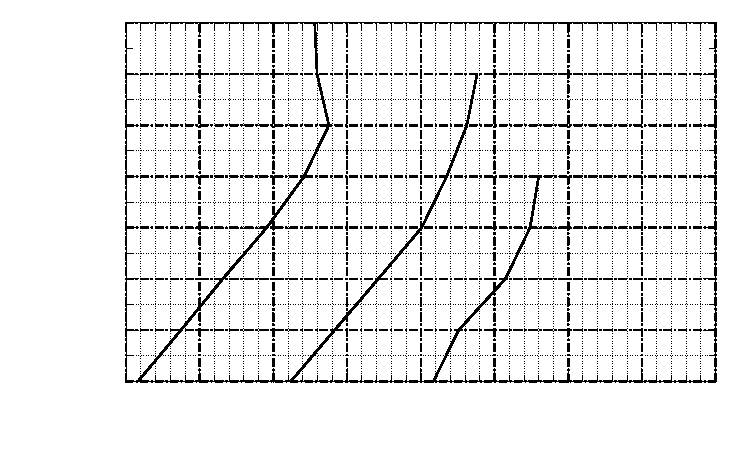
\includegraphics{../graphs/cruise_speed}}%
    \gplfronttext
  \end{picture}%
\endgroup
\end{center}  % for gnuplot epslatex, latex or pslatex mode
\caption{Cruise Speed}
\label{Cruise-speed}
\end{figure}


  % Cruise Speed Chart - Wheel Pants ON
% Cruise Speed Chart - Wheel Pants OFF
\begin{figure}[t]
% \addcontentsline{toc}{section}{Figure \ref{Cruise-speed} Cruise Speed}
\addcontentsline{toc}{section}{CRUISE SPEED - WHEEL PANTS OFF}
\begin{center}
\begin{perfhdr}CRUISE SPEED - WHEEL PANTS OFF\\
\end{perfhdr}

\begin{minipage}{5in}
  \begin{flushleft}
    CONDITIONS:\\
    Wheel Pants OFF, Gear Leg Fairings ON\\
    Standard atmosphere.\\
    Mixture set to best power for 75\% power.\\
    Mixture set to 50\textdegree F lean of peak EGT for 65\% and 55\% power.\\
    Full throttle.\\
    RPM set to obtain desired power, but no higher than 2700 rpm.\\
    \end{flushleft}
\end{minipage}\\
\vspace{5ex}

% GNUPLOT: LaTeX picture with Postscript
\begingroup
  \makeatletter
  \providecommand\color[2][]{%
    \GenericError{(gnuplot) \space\space\space\@spaces}{%
      Package color not loaded in conjunction with
      terminal option `colourtext'%
    }{See the gnuplot documentation for explanation.%
    }{Either use 'blacktext' in gnuplot or load the package
      color.sty in LaTeX.}%
    \renewcommand\color[2][]{}%
  }%
  \providecommand\includegraphics[2][]{%
    \GenericError{(gnuplot) \space\space\space\@spaces}{%
      Package graphicx or graphics not loaded%
    }{See the gnuplot documentation for explanation.%
    }{The gnuplot epslatex terminal needs graphicx.sty or graphics.sty.}%
    \renewcommand\includegraphics[2][]{}%
  }%
  \providecommand\rotatebox[2]{#2}%
  \@ifundefined{ifGPcolor}{%
    \newif\ifGPcolor
    \GPcolorfalse
  }{}%
  \@ifundefined{ifGPblacktext}{%
    \newif\ifGPblacktext
    \GPblacktexttrue
  }{}%
  % define a \g@addto@macro without @ in the name:
  \let\gplgaddtomacro\g@addto@macro
  % define empty templates for all commands taking text:
  \gdef\gplbacktext{}%
  \gdef\gplfronttext{}%
  \makeatother
  \ifGPblacktext
    % no textcolor at all
    \def\colorrgb#1{}%
    \def\colorgray#1{}%
  \else
    % gray or color?
    \ifGPcolor
      \def\colorrgb#1{\color[rgb]{#1}}%
      \def\colorgray#1{\color[gray]{#1}}%
      \expandafter\def\csname LTw\endcsname{\color{white}}%
      \expandafter\def\csname LTb\endcsname{\color{black}}%
      \expandafter\def\csname LTa\endcsname{\color{black}}%
      \expandafter\def\csname LT0\endcsname{\color[rgb]{1,0,0}}%
      \expandafter\def\csname LT1\endcsname{\color[rgb]{0,1,0}}%
      \expandafter\def\csname LT2\endcsname{\color[rgb]{0,0,1}}%
      \expandafter\def\csname LT3\endcsname{\color[rgb]{1,0,1}}%
      \expandafter\def\csname LT4\endcsname{\color[rgb]{0,1,1}}%
      \expandafter\def\csname LT5\endcsname{\color[rgb]{1,1,0}}%
      \expandafter\def\csname LT6\endcsname{\color[rgb]{0,0,0}}%
      \expandafter\def\csname LT7\endcsname{\color[rgb]{1,0.3,0}}%
      \expandafter\def\csname LT8\endcsname{\color[rgb]{0.5,0.5,0.5}}%
    \else
      % gray
      \def\colorrgb#1{\color{black}}%
      \def\colorgray#1{\color[gray]{#1}}%
      \expandafter\def\csname LTw\endcsname{\color{white}}%
      \expandafter\def\csname LTb\endcsname{\color{black}}%
      \expandafter\def\csname LTa\endcsname{\color{black}}%
      \expandafter\def\csname LT0\endcsname{\color{black}}%
      \expandafter\def\csname LT1\endcsname{\color{black}}%
      \expandafter\def\csname LT2\endcsname{\color{black}}%
      \expandafter\def\csname LT3\endcsname{\color{black}}%
      \expandafter\def\csname LT4\endcsname{\color{black}}%
      \expandafter\def\csname LT5\endcsname{\color{black}}%
      \expandafter\def\csname LT6\endcsname{\color{black}}%
      \expandafter\def\csname LT7\endcsname{\color{black}}%
      \expandafter\def\csname LT8\endcsname{\color{black}}%
    \fi
  \fi
  \setlength{\unitlength}{0.0500bp}%
  \begin{picture}(7200.00,5040.00)%
    \gplgaddtomacro\gplbacktext{%
      \csname LTb\endcsname%
      \put(1342,704){\makebox(0,0)[r]{\strut{}0}}%
      \csname LTb\endcsname%
      \put(1342,1286){\makebox(0,0)[r]{\strut{}2,000}}%
      \csname LTb\endcsname%
      \put(1342,1867){\makebox(0,0)[r]{\strut{}4,000}}%
      \csname LTb\endcsname%
      \put(1342,2449){\makebox(0,0)[r]{\strut{}6,000}}%
      \csname LTb\endcsname%
      \put(1342,3030){\makebox(0,0)[r]{\strut{}8,000}}%
      \csname LTb\endcsname%
      \put(1342,3612){\makebox(0,0)[r]{\strut{}10,000}}%
      \csname LTb\endcsname%
      \put(1342,4193){\makebox(0,0)[r]{\strut{}12,000}}%
      \csname LTb\endcsname%
      \put(1342,4775){\makebox(0,0)[r]{\strut{}14,000}}%
      \csname LTb\endcsname%
      \put(1474,484){\makebox(0,0){\strut{} 135}}%
      \csname LTb\endcsname%
      \put(2148,484){\makebox(0,0){\strut{} 140}}%
      \csname LTb\endcsname%
      \put(2823,484){\makebox(0,0){\strut{} 145}}%
      \csname LTb\endcsname%
      \put(3497,484){\makebox(0,0){\strut{} 150}}%
      \csname LTb\endcsname%
      \put(4172,484){\makebox(0,0){\strut{} 155}}%
      \csname LTb\endcsname%
      \put(4846,484){\makebox(0,0){\strut{} 160}}%
      \csname LTb\endcsname%
      \put(5520,484){\makebox(0,0){\strut{} 165}}%
      \csname LTb\endcsname%
      \put(6195,484){\makebox(0,0){\strut{} 170}}%
      \csname LTb\endcsname%
      \put(6869,484){\makebox(0,0){\strut{} 175}}%
      \put(308,2739){\rotatebox{-270}{\makebox(0,0){\strut{}Altitude (ft)}}}%
      \put(4171,154){\makebox(0,0){\strut{}Cruise Speed - Wheel Pants OFF (KTAS)}}%
      \put(5224,1286){\rotatebox{55}{\makebox(0,0)[l]{\strut{}75\% Power}}}%
      \put(4536,1722){\rotatebox{55}{\makebox(0,0)[l]{\strut{}65\% Power}}}%
      \put(3726,2158){\rotatebox{56}{\makebox(0,0)[l]{\strut{}55\% Power}}}%
      \put(1528,4612){\makebox(0,0)[l]{\strut{}From Flight Tests 20 \& 22 Jan 2011}}%
    }%
    \gplgaddtomacro\gplfronttext{%
    }%
    \gplbacktext
    \put(0,0){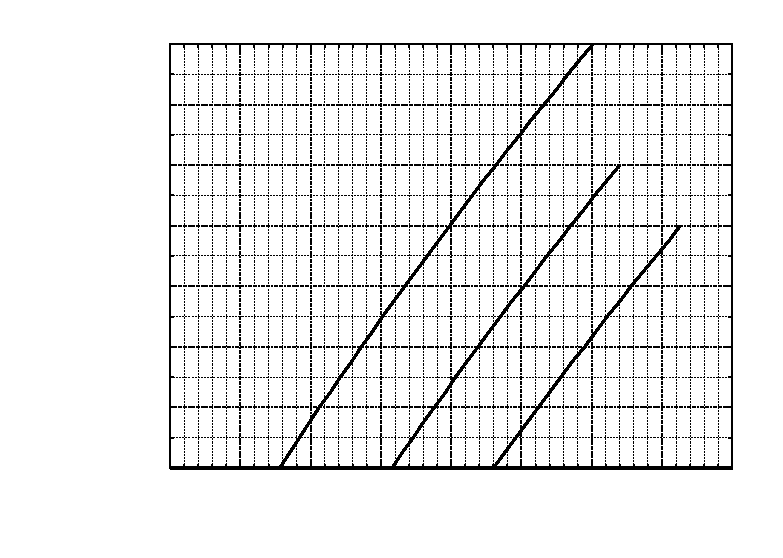
\includegraphics{../graphs/cruise_speed_wheel_pants_off}}%
    \gplfronttext
  \end{picture}%
\endgroup
\end{center}  % for gnuplot epslatex, latex or pslatex mode
\caption{Cruise Speed - Wheel Pants OFF}
\label{Cruise-speed-WP-OFF}
\end{figure}


 % Cruise Speed Chart - Wheel Pants OFF
% Cruise Range Chart - Wheel Pants ON
\begin{figure}[t]
% \addcontentsline{toc}{section}{Figure \ref{Cruise-range} Cruise Range}
\addcontentsline{toc}{section}{CRUISE RANGE}
\begin{center}
\begin{perfhdr}CRUISE RANGE\\
\end{perfhdr}

\begin{minipage}{5in}
  \begin{flushleft}
    CONDITIONS:\\
    Wheel Pants and Gear Leg Fairings ON\\
    43 USG Usable Fuel.\\
    Standard atmosphere.\\
    No wind.\\
    Includes 1.0 USG fuel for start, taxi and takeoff and 8 USG or 45 mn reserve.\\
    Climb at full power and best climb speed as defined on the Maximum Climb Chart\\
    Lean during climb for best power.\\
    Cruise with mixture set to best power for 75\% power.  Mixture set to 50\textdegree F lean of peak EGT for 65\% or less, except mixture set to best power if more than 2600 rpm required with mixture set lean of peak EGT.\\
    Full throttle, but no less than 2100 rpm.\\
    Descend at cruise TAS at 6 nm per 1000 ft.\\
    \end{flushleft}
\end{minipage}\\
\vspace{5ex}
% GNUPLOT: LaTeX picture with Postscript
\begingroup
  \makeatletter
  \providecommand\color[2][]{%
    \GenericError{(gnuplot) \space\space\space\@spaces}{%
      Package color not loaded in conjunction with
      terminal option `colourtext'%
    }{See the gnuplot documentation for explanation.%
    }{Either use 'blacktext' in gnuplot or load the package
      color.sty in LaTeX.}%
    \renewcommand\color[2][]{}%
  }%
  \providecommand\includegraphics[2][]{%
    \GenericError{(gnuplot) \space\space\space\@spaces}{%
      Package graphicx or graphics not loaded%
    }{See the gnuplot documentation for explanation.%
    }{The gnuplot epslatex terminal needs graphicx.sty or graphics.sty.}%
    \renewcommand\includegraphics[2][]{}%
  }%
  \providecommand\rotatebox[2]{#2}%
  \@ifundefined{ifGPcolor}{%
    \newif\ifGPcolor
    \GPcolorfalse
  }{}%
  \@ifundefined{ifGPblacktext}{%
    \newif\ifGPblacktext
    \GPblacktexttrue
  }{}%
  % define a \g@addto@macro without @ in the name:
  \let\gplgaddtomacro\g@addto@macro
  % define empty templates for all commands taking text:
  \gdef\gplbacktext{}%
  \gdef\gplfronttext{}%
  \makeatother
  \ifGPblacktext
    % no textcolor at all
    \def\colorrgb#1{}%
    \def\colorgray#1{}%
  \else
    % gray or color?
    \ifGPcolor
      \def\colorrgb#1{\color[rgb]{#1}}%
      \def\colorgray#1{\color[gray]{#1}}%
      \expandafter\def\csname LTw\endcsname{\color{white}}%
      \expandafter\def\csname LTb\endcsname{\color{black}}%
      \expandafter\def\csname LTa\endcsname{\color{black}}%
      \expandafter\def\csname LT0\endcsname{\color[rgb]{1,0,0}}%
      \expandafter\def\csname LT1\endcsname{\color[rgb]{0,1,0}}%
      \expandafter\def\csname LT2\endcsname{\color[rgb]{0,0,1}}%
      \expandafter\def\csname LT3\endcsname{\color[rgb]{1,0,1}}%
      \expandafter\def\csname LT4\endcsname{\color[rgb]{0,1,1}}%
      \expandafter\def\csname LT5\endcsname{\color[rgb]{1,1,0}}%
      \expandafter\def\csname LT6\endcsname{\color[rgb]{0,0,0}}%
      \expandafter\def\csname LT7\endcsname{\color[rgb]{1,0.3,0}}%
      \expandafter\def\csname LT8\endcsname{\color[rgb]{0.5,0.5,0.5}}%
    \else
      % gray
      \def\colorrgb#1{\color{black}}%
      \def\colorgray#1{\color[gray]{#1}}%
      \expandafter\def\csname LTw\endcsname{\color{white}}%
      \expandafter\def\csname LTb\endcsname{\color{black}}%
      \expandafter\def\csname LTa\endcsname{\color{black}}%
      \expandafter\def\csname LT0\endcsname{\color{black}}%
      \expandafter\def\csname LT1\endcsname{\color{black}}%
      \expandafter\def\csname LT2\endcsname{\color{black}}%
      \expandafter\def\csname LT3\endcsname{\color{black}}%
      \expandafter\def\csname LT4\endcsname{\color{black}}%
      \expandafter\def\csname LT5\endcsname{\color{black}}%
      \expandafter\def\csname LT6\endcsname{\color{black}}%
      \expandafter\def\csname LT7\endcsname{\color{black}}%
      \expandafter\def\csname LT8\endcsname{\color{black}}%
    \fi
  \fi
  \setlength{\unitlength}{0.0500bp}%
  \begin{picture}(7200.00,5040.00)%
    \gplgaddtomacro\gplbacktext{%
      \csname LTb\endcsname%
      \put(1342,704){\makebox(0,0)[r]{\strut{}0}}%
      \csname LTb\endcsname%
      \put(1342,1286){\makebox(0,0)[r]{\strut{}2,000}}%
      \csname LTb\endcsname%
      \put(1342,1867){\makebox(0,0)[r]{\strut{}4,000}}%
      \csname LTb\endcsname%
      \put(1342,2449){\makebox(0,0)[r]{\strut{}6,000}}%
      \csname LTb\endcsname%
      \put(1342,3030){\makebox(0,0)[r]{\strut{}8,000}}%
      \csname LTb\endcsname%
      \put(1342,3612){\makebox(0,0)[r]{\strut{}10,000}}%
      \csname LTb\endcsname%
      \put(1342,4193){\makebox(0,0)[r]{\strut{}12,000}}%
      \csname LTb\endcsname%
      \put(1342,4775){\makebox(0,0)[r]{\strut{}14,000}}%
      \csname LTb\endcsname%
      \put(1474,484){\makebox(0,0){\strut{} 500}}%
      \csname LTb\endcsname%
      \put(2823,484){\makebox(0,0){\strut{} 550}}%
      \csname LTb\endcsname%
      \put(4172,484){\makebox(0,0){\strut{} 600}}%
      \csname LTb\endcsname%
      \put(5520,484){\makebox(0,0){\strut{} 650}}%
      \csname LTb\endcsname%
      \put(6869,484){\makebox(0,0){\strut{} 700}}%
      \put(308,2739){\rotatebox{-270}{\makebox(0,0){\strut{}Altitude (ft)}}}%
      \put(4171,154){\makebox(0,0){\strut{}Cruise Range (NM)}}%
      \put(3227,1373){\rotatebox{77}{\makebox(0,0)[l]{\strut{}75\% Power}}}%
      \put(4576,1727){\rotatebox{76}{\makebox(0,0)[l]{\strut{}65\% Power}}}%
      \put(6060,2158){\rotatebox{76}{\makebox(0,0)[l]{\strut{}55\% Power}}}%
      \put(4172,3874){\makebox(0,0){\strut{}\Large\textcolor{red}{FROM ANALYSIS OF CAFE DATA}\normalsize}}%
      \put(4172,3292){\makebox(0,0){\strut{}\Large\textcolor{red}{PENDING FLIGHT TEST}\normalsize}}%
    }%
    \gplgaddtomacro\gplfronttext{%
    }%
    \gplbacktext
    \put(0,0){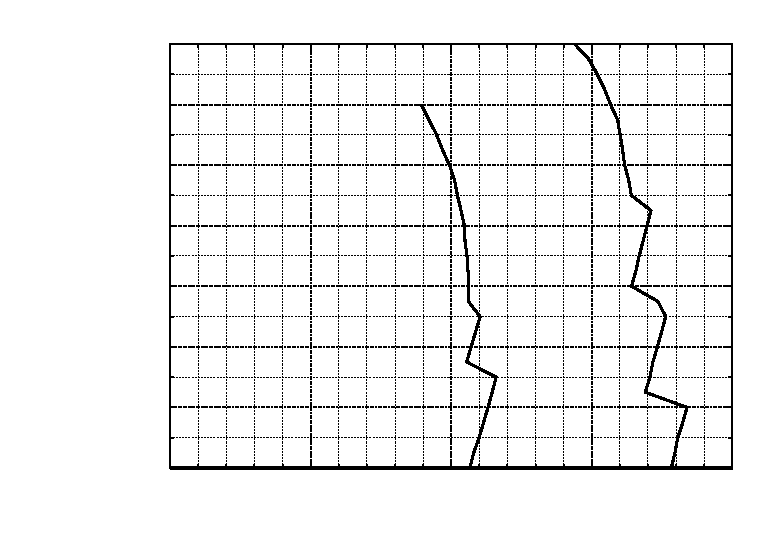
\includegraphics{../graphs/cruise_range}}%
    \gplfronttext
  \end{picture}%
\endgroup
\end{center}  % for gnuplot epslatex, latex or pslatex mode
\caption{Cruise Range}
\label{Cruise-range}
\end{figure}
\clearpage


     % Cruise Range Chart - Wheel Pants ON
% Cruise Range Chart - Wheel Pants OFF
\begin{figure}[t]
% \addcontentsline{toc}{section}{Figure \ref{Cruise-range} Cruise Range}
\addcontentsline{toc}{section}{CRUISE RANGE - WHEEL PANTS OFF}
\begin{center}
\begin{perfhdr}CRUISE RANGE - WHEEL PANTS OFF\\
\end{perfhdr}

\begin{minipage}{5in}
  \begin{flushleft}
    CONDITIONS:\\
    Wheel Pants OFF, Gear Leg Fairings ON\\
    43 USG Usable Fuel.\\
    Standard atmosphere.\\
    No wind.\\
    Includes 1.0 USG fuel for start, taxi and takeoff and 8 USG or 45 mn reserve.\\
    Climb at full power and best climb speed as defined on the Maximum Climb Chart\\
    Lean during climb for best power.\\
    Cruise with mixture set to best power for 75\% power.  \\
    Cruise with mixture set to 50\textdegree F lean of peak EGT for 65\% power or less, except mixture set to best power if more than 2600 rpm required with mixture set lean of peak EGT.\\
    Descend at cruise TAS at 6 nm per 1000 ft.\\
    \end{flushleft}
\end{minipage}\\
\vspace{5ex}
% GNUPLOT: LaTeX picture with Postscript
\begingroup
  \makeatletter
  \providecommand\color[2][]{%
    \GenericError{(gnuplot) \space\space\space\@spaces}{%
      Package color not loaded in conjunction with
      terminal option `colourtext'%
    }{See the gnuplot documentation for explanation.%
    }{Either use 'blacktext' in gnuplot or load the package
      color.sty in LaTeX.}%
    \renewcommand\color[2][]{}%
  }%
  \providecommand\includegraphics[2][]{%
    \GenericError{(gnuplot) \space\space\space\@spaces}{%
      Package graphicx or graphics not loaded%
    }{See the gnuplot documentation for explanation.%
    }{The gnuplot epslatex terminal needs graphicx.sty or graphics.sty.}%
    \renewcommand\includegraphics[2][]{}%
  }%
  \providecommand\rotatebox[2]{#2}%
  \@ifundefined{ifGPcolor}{%
    \newif\ifGPcolor
    \GPcolorfalse
  }{}%
  \@ifundefined{ifGPblacktext}{%
    \newif\ifGPblacktext
    \GPblacktexttrue
  }{}%
  % define a \g@addto@macro without @ in the name:
  \let\gplgaddtomacro\g@addto@macro
  % define empty templates for all commands taking text:
  \gdef\gplbacktext{}%
  \gdef\gplfronttext{}%
  \makeatother
  \ifGPblacktext
    % no textcolor at all
    \def\colorrgb#1{}%
    \def\colorgray#1{}%
  \else
    % gray or color?
    \ifGPcolor
      \def\colorrgb#1{\color[rgb]{#1}}%
      \def\colorgray#1{\color[gray]{#1}}%
      \expandafter\def\csname LTw\endcsname{\color{white}}%
      \expandafter\def\csname LTb\endcsname{\color{black}}%
      \expandafter\def\csname LTa\endcsname{\color{black}}%
      \expandafter\def\csname LT0\endcsname{\color[rgb]{1,0,0}}%
      \expandafter\def\csname LT1\endcsname{\color[rgb]{0,1,0}}%
      \expandafter\def\csname LT2\endcsname{\color[rgb]{0,0,1}}%
      \expandafter\def\csname LT3\endcsname{\color[rgb]{1,0,1}}%
      \expandafter\def\csname LT4\endcsname{\color[rgb]{0,1,1}}%
      \expandafter\def\csname LT5\endcsname{\color[rgb]{1,1,0}}%
      \expandafter\def\csname LT6\endcsname{\color[rgb]{0,0,0}}%
      \expandafter\def\csname LT7\endcsname{\color[rgb]{1,0.3,0}}%
      \expandafter\def\csname LT8\endcsname{\color[rgb]{0.5,0.5,0.5}}%
    \else
      % gray
      \def\colorrgb#1{\color{black}}%
      \def\colorgray#1{\color[gray]{#1}}%
      \expandafter\def\csname LTw\endcsname{\color{white}}%
      \expandafter\def\csname LTb\endcsname{\color{black}}%
      \expandafter\def\csname LTa\endcsname{\color{black}}%
      \expandafter\def\csname LT0\endcsname{\color{black}}%
      \expandafter\def\csname LT1\endcsname{\color{black}}%
      \expandafter\def\csname LT2\endcsname{\color{black}}%
      \expandafter\def\csname LT3\endcsname{\color{black}}%
      \expandafter\def\csname LT4\endcsname{\color{black}}%
      \expandafter\def\csname LT5\endcsname{\color{black}}%
      \expandafter\def\csname LT6\endcsname{\color{black}}%
      \expandafter\def\csname LT7\endcsname{\color{black}}%
      \expandafter\def\csname LT8\endcsname{\color{black}}%
    \fi
  \fi
  \setlength{\unitlength}{0.0500bp}%
  \begin{picture}(7200.00,5040.00)%
    \gplgaddtomacro\gplbacktext{%
      \csname LTb\endcsname%
      \put(1210,704){\makebox(0,0)[r]{\strut{}0}}%
      \csname LTb\endcsname%
      \put(1210,1722){\makebox(0,0)[r]{\strut{}5,000}}%
      \csname LTb\endcsname%
      \put(1210,2740){\makebox(0,0)[r]{\strut{}10,000}}%
      \csname LTb\endcsname%
      \put(1210,3757){\makebox(0,0)[r]{\strut{}15,000}}%
      \csname LTb\endcsname%
      \put(1210,4775){\makebox(0,0)[r]{\strut{}20,000}}%
      \csname LTb\endcsname%
      \put(1342,484){\makebox(0,0){\strut{} 450}}%
      \csname LTb\endcsname%
      \put(1949,484){\makebox(0,0){\strut{} 500}}%
      \csname LTb\endcsname%
      \put(2556,484){\makebox(0,0){\strut{} 550}}%
      \csname LTb\endcsname%
      \put(3162,484){\makebox(0,0){\strut{} 600}}%
      \csname LTb\endcsname%
      \put(3769,484){\makebox(0,0){\strut{} 650}}%
      \csname LTb\endcsname%
      \put(4376,484){\makebox(0,0){\strut{} 700}}%
      \csname LTb\endcsname%
      \put(4983,484){\makebox(0,0){\strut{} 750}}%
      \csname LTb\endcsname%
      \put(5589,484){\makebox(0,0){\strut{} 800}}%
      \csname LTb\endcsname%
      \put(6196,484){\makebox(0,0){\strut{} 850}}%
      \csname LTb\endcsname%
      \put(6803,484){\makebox(0,0){\strut{} 900}}%
      \put(176,2739){\rotatebox{-270}{\makebox(0,0){\strut{}Altitude (ft)}}}%
      \put(4072,154){\makebox(0,0){\strut{}Cruise Range - Wheel Pants OFF (NM)}}%
      \put(1762,1009){\rotatebox{83}{\makebox(0,0)[l]{\strut{}75\% Power}}}%
      \put(3512,1213){\rotatebox{88}{\makebox(0,0)[l]{\strut{}65\% Power}}}%
      \put(4265,1213){\rotatebox{73}{\makebox(0,0)[l]{\strut{}55\% Power}}}%
      \put(5036,1213){\rotatebox{71}{\makebox(0,0)[l]{\strut{}45\% Power}}}%
      \put(5700,1213){\rotatebox{71}{\makebox(0,0)[l]{\strut{}35\% Power}}}%
    }%
    \gplgaddtomacro\gplfronttext{%
    }%
    \gplbacktext
    \put(0,0){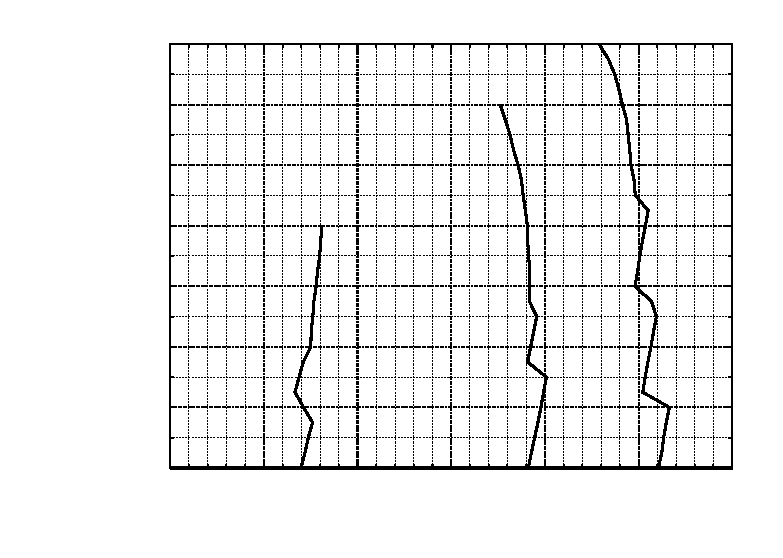
\includegraphics{../graphs/cruise_range_wheel_pants_off}}%
    \gplfronttext
  \end{picture}%
\endgroup
\end{center}  % for gnuplot epslatex, latex or pslatex mode
\caption{Cruise Range - Wheel Pants OFF}
\label{Cruise-range-WP-OFF}
\end{figure}
\clearpage


    % Cruise Range Chart - Wheel Pants OFF
% Landing Distance
\begin{sidewaysfigure}[t]
% \addcontentsline{toc}{section}{Figure \ref{Landing-dist} Landing Distance}
\addcontentsline{toc}{section}{LANDING DISTANCE}
\begin{center}
\begin{perfhdr}LANDING DISTANCE\\
1800 LBS
\end{perfhdr}
\Large
\textcolor{red}{VANS CLAIMED PERF EXPANDED TO OTHER CONDITIONS}\vspace{1ex}\\
\textcolor{red}{TO BE CONFIRMED BY FLIGHT TEST}\normalsize \vspace{5ex}\\

\begin{minipage}{9in}
  \begin{flushleft}
    CONDITIONS:\\
    Full Flaps\\
    Power OFF\\
    Maximum Braking\\
    Paved, Level, Dry Runway\\
    Zero Wind\\

    NOTES:
    \begin{enumerate*}
      \item Short field technique as specified in Section \textcolor{red}{4}.
      \item Decrease distances by 10\% for each 5 knots headwind.  For operations with tailwinds up to 10 knots, increase distances by 10\% for each 2 knots.
      \item For operation on a dry, grass runway, increase distances by 40\% of the ground roll figure.
      \end{enumerate*}
    \end{flushleft}
\end{minipage}\\

\vspace{\perfnoteskip}

\settowidth{\colOne}{WEIGHT}
\settowidth{\colTwo}{SPEED}
\settowidth{\colThree}{PRESS}
\settowidth{\colFour}{GRND}
\settowidth{\colFive}{TOTAL}
\setlength{\rowdrop}{\baselineskip/-1}
\begin{tabular}{|c|c|r|r|r|r|r|r|r|r|r|r|r|}
\hline
\multirow{5}{\colOne}{\centering WEIGHT (LB)}&\multirow{5}{\colTwo}{\centering SPEED AT 50 FT (KIAS)}&
\multirow{5}{\colThree}{\centering PRESS ALT (FT)}&\multicolumn{2}{c|}{0\textdegree C}&
\multicolumn{2}{c|}{10\textdegree C}&\multicolumn{2}{c|}{20\textdegree C}&
\multicolumn{2}{c|}{30\textdegree C}&\multicolumn{2}{c|}{40\textdegree C}\\
\cline{4-13}
&&&\multirow{4}{\colFour}{\centering GRND ROLL (FT)}&\multirow{4}{\colFive}{\centering TOTAL DIST FROM 50 FT}&
\multirow{4}{\colFour}{\centering GRND ROLL (FT)}&\multirow{4}{\colFive}{\centering TOTAL DIST FROM 50 FT}&
\multirow{4}{\colFour}{\centering GRND ROLL (FT)}&\multirow{4}{\colFive}{\centering TOTAL DIST FROM 50 FT}&
\multirow{4}{\colFour}{\centering GRND ROLL (FT)}&\multirow{4}{\colFive}{\centering TOTAL DIST FROM 50 FT}&
\multirow{4}{\colFour}{\centering GRND ROLL (FT)}&\multirow{4}{\colFive}{\centering TOTAL DIST FROM 50 FT}\\
&&&&&&&&&&&&\\ 
&&&&&&&&&&&&\\
&&&&&&&&&&&&\\
\hline
\hline

1800&XX&S.L.&470&TTT&490&TTT&510&TTT&530&TTT&540&TTT\\
\hline
&XX&2,000&510&TTT&530&TTT&550&TTT&570&TTT&580&TTT\\
\hline
&XX&4,000&550&TTT&570&TTT&590&TTT&610&TTT&630&TTT\\
\hline
&XX&6,000&590&TTT&610&TTT&630&TTT&660&TTT&680&TTT\\
\hline
&XX&8,000&640&TTT&660&TTT&680&TTT&710&TTT&730&TTT\\
\hline
&XX&10,000&690&TTT&710&TTT&740&TTT&760&TTT&790&TTT\\
\hline
&XX&12,000&750&TTT&770&TTT&800&TTT&830&TTT&850&TTT\\
\hline
\end{tabular}
\end{center}
\caption{Landing Distance}
\label{Landing-dist}
\end{sidewaysfigure}

                % Landing Distance


\clearpage

\textcolor{red}{To be added once flight test data is available:
\begin{enumerate*}
\item Airspeed Calibration --- Normal Static Source --- Flaps Extended
\item Airspeed Calibration --- Alternate Static Source --- All Flap Positions
\item Altitude Calibration --- Normal Static Source --- Flaps Extended
\item Altitude Calibration --- Alternate Static Source --- All Flap Positions
\item Stall Speeds --- IAS
%\item Range Profile
\item Holding Speed and Fuel Flow
\item Endurance Profile
\end{enumerate*}}
\cleardoublepage
